\documentclass{ruthesis}
\usepackage{graphicx}          % Include this line if your
                               % document contains figures,
%\usepackage[dvips]{epsfig}    % or this line, depending on which
                               % you prefer.

\usepackage{listings}
\lstset{breaklines=true}
\lstset{numbers=left, numberstyle=\scriptsize\ttfamily, numbersep=10pt, captionpos=b} 
\lstset{basicstyle=\small\ttfamily}
\lstset{framesep=4pt}
\usepackage{amsfonts,amssymb,amsbsy}
\usepackage{latexsym}
\usepackage{amsmath}
\usepackage{color}
\usepackage{graphics} % for pdf, bitmapped graphics files
\usepackage{epsfig} % for postscript graphics files
\usepackage{epstopdf}
\usepackage{caption}
\usepackage{subcaption}
\usepackage{longtable}
\usepackage{multirow}
\usepackage{afterpage}
\usepackage{array,booktabs,enumitem}% http://ctan.org/pkg/
\newcolumntype{P}[1]{>{\endgraf\vspace*{-\baselineskip}}p{#1}}
%\usepackage{graphicx,subfigure}
%\usepackage{rotating}
%\usepackage{theorem}
%%\usepackage{isomath}
%\usepackage{mathrsfs}
%\usepackage{enumerate}

\usepackage{placeins}
\usepackage{rotating}
\usepackage{titlesec}
\usepackage{geometry}
 \geometry{
 a4paper,
 total={210mm,297mm}, left=20mm, right=20mm, top=20mm, bottom=20mm,}
 
\def\etal{\mbox{et al.}}
\DeclareMathOperator*{\sign}{sign}
\DeclareMathOperator*{\diag}{diag}
\DeclareMathOperator*{\proj}{proj}
\DeclareMathOperator*{\argmin}{argmin}
\DeclareMathOperator*{\rank}{rank}
\newcommand{\norm}[1]{{{\lVert #1 \rVert}}}
\newcommand{\clN}{{\cal N}}
\newcommand{\clM}{{\cal M}}
%\newcommand{\diag}{{\sf diag}}
%\newcommand{\sgn}{{\sf sgn}}
\newtheorem{proposition}{Proposition}
\newtheorem{theorem}{Theorem}
\newtheorem{lemma}{Lemma}
\newtheorem{corollary}{Corollary}
\newtheorem{remark}{Remark}
\newtheorem{definition}{Definition}
\newtheorem{assumption}{Assumption}

\setlength{\parskip}{0.2cm} 
\setlength{\topmargin}{-0.4cm}
\setlength{\oddsidemargin}{1cm} 
\setlength\evensidemargin{1cm}
\setlength{\textwidth}{15cm} 
\setlength{\textheight}{23.5cm}
\titlespacing\section{-4pt}{12pt plus 4pt minus 2pt}{0pt plus 2pt minus 2pt}
\titlespacing\subsection{0pt}{12pt plus 4pt minus 2pt}{0pt plus 2pt minus 2pt}
\titlespacing\subsubsection{0pt}{12pt plus 4pt minus 2pt}{0pt plus 2pt minus 2pt}
\titleformat{\subsubsection}
  {\bfseries\itshape\normalsize}{\thesubsubsection}{1em}{}

\begin{document}
\tableofcontents

\pagenumbering{arabic}
\linespacing{1.7}

\setcounter{chapter}{3}
\chapter{A data assimilating state-space model for algal growth under controlled conditions within a photo-bioreactor}\label{ch:Intro}


\section{Introduction}\label{sec:micro_intro} 

The key goal of biofuels production is the optimisation of biomass productivity in large-scale microalgal culturing systems such as open ponds or closed photo‐bioreactors.

Carbon and light availability are two of the most common limiting factors of biomass productivity \cite{posten2009design}.



%[BM for ref: At 2 hour intervals, a solenoid valve (SMC Pneumatics Pty. Ltd.) was used to stop aeration for 10 minutes. The linear increase in DO caused by these artefacts were used to calculate net photosynthesis. (reference Tamburic 2015)]





\section{Methods}

\subsection{Data Model: Photo-bioreactor setup, experimental design and data collection methods}

All data collection methods for this chapter were carried out by Peter Wood as part of a collection of PhD experiments (Peter Wood 2019 UTS PhD).

Microalgal culture \emph{Nannochloropsis oceanica} (Droop) Green (strain CS-179) obtained from the Australian National Algae Culture Collection was cultured in 200$\mskip3mu$mL conical flasks; maintained in an incubator (Labec Pty Ltd) at 20$^{\circ}$C, under an irradiance of
50$\mskip3mu$$\mu$mol$\mskip3mu$m$^{-2}$$\mskip3mu$s$^{-1}$ of cool-white fluorescent light at a 12 hour light/12 hour dark cycle. Stock cultures were grown in f/2 saltwater medium \cite{guillard1962studies} and diluted 5 days prior to the start of experiments to ensure that \emph{N. oceanica} was in the exponential growth phase and not nutrient deprived. f/2 was sparged prior to stock culture dilutions to maximise carbon and oxygen content.  

\emph{N. oceanica} was cultured in four, 500$\mskip3mu$mL environmental photo-bioreactors (ePBRs, Phenometrics Inc) with a 10\% v/v inoculation of stock culture. Top-side illumination over a path length of 25$\mskip3mu$cm was provided by a cool-white light LED, whilst temperature was maintained at 27$^{\circ}$C using a Peltier heater-cooler connected to a water jacket. In-built thermocouples, calibrated against external temperature sensors attached to the Firesting module (TeX4; PyroScience GmbH), measured every 5 minutes were used to control the Peltier heater-cooler jacket through a feedback loop to an accuracy of $\pm$ 0.2$^{\circ}$C. pH was also measured in 5 min intervals by in-built pH electrodes (Van London Inc); controlled by periodic CO2 (5\%) injections using valves in the ePBRs. pH was 3-point calibrated using pH buffer solutions at pH 4.00 $\pm$ 0.02, pH 7.00 $\pm$ 0.02 and pH 10.00 $\pm$ 0.02.  PBR mixing was controlled by magnetic stirring bars at 110 rpm. All four ePBRs were aerated with filtered/humidified air through a 1.2$\mskip3mu$mm needle valve (Terumo Co). 


A period of 2 days was allowed for \emph{N. occulata} to acclimate to the ePBRs at an irradiance of 500$\mskip3mu$$\mu$mol$\mskip3mu$m$^{-2}$$\mskip3mu$s$^{-1}$ and a temperature of 27$^{\circ}$C. Following this acclimation period, the PBR was set to the experimental condition of 2,000$\mskip3mu$$\mu$mol$\mskip3mu$photons$\mskip3mu$m$^{-2}$$\mskip3mu$s$^{-1}$ for another 2 days and a 12 hour light/12 hour dark cycle with a temperature of 27$^{\circ}$C. 
ePBRs were maintained at an optical density (OD) of 0.4 using manual dilutions, creating a semi-batch culturing system. Dilutions occurred once per day (one hour before the light cycle), using aerated f/2 media. The experiment was conducted over a period of 4 days, samples were extracted post and prior dilution, as well as half way through the light cycle. %2$\mskip3mu$mL samples were extracted to measure: OD$_{750}$, cell density, nitrogen concentration and phosphorous concentration. 50$\mskip3mu$mL was extracted to examine alkalinity, dry weight, carbon percentage and nitrogen percentage. 
50$\mskip3mu$mL was extracted to examine total alkalinity and dissolved inorganic carbon. 
%Both pH and DO were measured every 5 mins and 1 min respectively; to generate dynamic daily profiles. 
Dissolved oxygen (DO) was measured using a 3$\mskip3mu$mm robust optical probe (OXROB10-OI; PyroScience GmbH) attached to a FireStingO2 logger (PyroScience GmbH). DO measurements were taken every 60 seconds and temperature-corrected using a temperature extension module (TeX4; PyroScience GmbH). DO was two-point calibrated using air-saturated seawater (100\% saturation) and sodium sulfate-saturated water (0\% saturation). At 2 hour intervals, a solenoid valve (SMC Pneumatics Pty. Ltd.) was used to stop aeration for 10 minutes to allow for observations of net photosynthesis. Alkalinity was measured twice a day using TA titration; 0.1$\mskip3mu$M hydrochloric acid on 30$\mskip3mu$mL of \emph{N. oceanica} media using an auto-titrator (800 Dosino; Metrohm AG). 

[Chris: DIC measurement collection description]

[BM: confirm that reference with PW]


\subsection{Data model: Data treatment, distributions and measurement error}

Valve, temperature, light (normalised to 0/1) and dilution rates were used to force the model.
Dissolved oxygen, pH, dissolved inorganic carbon and total alkalinity observations for 4 days post acclimation were assimilated. 
While pH observations were calibrated and corrected, it was visible that $O_2$ observations were not completely calibrated and experienced some sensor drift during the experiment. An offset term ($offset_{O_2}$) was added to the $O_2$ ode to account for this. The offset was assigned a normally distributed prior distribution with mean 0 and standard deviation 2. [BM:check the offset is still there and you did it this way otherwise change/remove.]

The data model assigned log normally distributed observation errors for each instrument;
$O_{2_{obs}}$ $\sim$ Log$\mathcal{N}$(log($O_2$), $\sigma_{O_2}$), $pH_{obs}$ $\sim$ Log$\mathcal{N}$(log($pH$),  $\sigma_{pH}$), $DIC_{obs}$ $\sim$ Log$\mathcal{N}$(log($DIC$), $\sigma_{DIC}$), $TA_{obs}$ $\sim$ Log$\mathcal{N}$(log($TA$), $\sigma_{DIC}$), where the standard deviations ($\sigma_{O_2}$, $\sigma_{pH}$, $\sigma_{DIC}$) were unknown parameters to be estimated as part of the assimilating model. Dissolved inorganic carbon and total alkalinity measurements were obtained from the same instrument thus the error is shared between these states. Initial observation error priors started at $\sigma_{O_2}$ $\sim$ Log$\mathcal{N}$(log(0.1), 0.5) and then were adjusted during the PMMH tuning phase. 


[Chris/SW: should I talk about the thinning out of $O_2$ and pH obs?]


\subsection{Process model: Carbon chemistry}

Ideally CO2SYS \cite{lewis1998program} would have been used to calculate the carbon chemistry of the photo-bioreactor. 
CO2SYS is a program developed for CO$_2$ system calculations (CO2SYS) that calculates and returns a detailed state of the carbonate system of oceanographic water samples in seawater and freshwater \cite{lewis1998program}.
Using two of the four measurable carbonate system parameters (total alkalinity, total inorganic CO$_2$, pH, and either fugacity fCO$_2$ or partial pressure of CO$_2$) to calculate the other two parameters at a set of input conditions (temperature and pressure). 

To incorporate CO2SYS into LiBbi for solving carbon chemistry on the timescale of the microalgae model, we explicitly defined 3 iterations (Eq. \ref{newton_raph_iterations1} - \ref{newton_raph_iterations_end}) of the Newton-Raphson method for finding approximations to roots of real valued functions. The Newton-Raphson method is an iterative process 
$ x_{n+1} = x_n - \frac{f(x_n)}{f'(x_n)} $
considering a function $f(x_n)$, its derivative $f'(x_n)$ and an initial starting value $x_0$. The approximate root $x_{n+1}$ converges to the exact solution very quickly if a close initial starting value is picked. To ensure the quick convergence of the Newton-Raphson method, an approximating equation for $pH_0$ (Eq. \ref{pH_approx_eq}) was obtained by fitting a stepwise regression with interactions to a range of simulated CO2SYS input parameters (temperature: 20-30, salinity: 30-40, $DIC$: 200-2500, and alkalinity: 1500-3000). A range of initial conditions and parameter values were tested, and each converged with RMSE $<$ 0.01 across $pH$, $HCO_3^-$, $CO_2$, and $CO_3$, $DIC$, $O_2$, $TA$ by the 3rd iteration (Figure \ref{fig:iterative_carbon_and_states} and Table \ref{table:rmse_iterative}).

%HCO$_3^-$, CO$_2$, and CO$_3$ were calculated from the 3rd iteration of pH.


\subsubsection{CO2SYS constants and iterative solution for pH, HCO$_3^-$, CO$_2$, and CO$_3$}

Total Sulfur:
\begin{align*}
TS     	&= \frac{0.14}{96.062} * \frac{S}{1.8065} \nonumber \\
IS     	&= 19.924 \frac{S}{(1000 - 1.005 S)} \nonumber \\
KS_{int} 	&= -\frac{4276.1}{T_K} + 141.328 - 23.093 log(T_K) + (-\frac{13856.0}{T_K} + 324.57 \nonumber\\ 			 
& - 47.986 log(T_K)) \sqrt{IS} + ( \frac{35474}{T_K} - 771.54  + 114.723 log(T_K)) IS \nonumber \\
& - \frac{2698}{T_K} IS^{1.5} + \frac{1776}{T_K} IS^2 \nonumber \\
KS     	&=  (1 - 0.001005 S)e^{(KS_{int})} \nonumber 
\end{align*}

Fluorine:
\begin{align*}
TF       	&= \frac{\frac{0.000067 S}{18.9984}}{1.80655} \nonumber \\
KF       	&= e^{(-(-\frac{874.0}{T_K} - 0.111 \sqrt{S} + 9.68))} \nonumber \\
SWS_{2_T}  	&= \frac{(1 + \frac{TS}{KS})}{(1 + \frac{TS}{KS} + \frac{TF}{KF})} \nonumber \\
Free_{2_T} 	&= 1 + \frac{TS}{KS} \nonumber 
\end{align*}

H2O dissoc:
\begin{align*}
KW 		&= e^{(148.9802 - \frac{13847.26}{T_K}  - 23.6521 log(T_K) 
+ (\frac{118.67}{T_K} - 5.977 + 1.0495 log(T_K)) \sqrt{S} - 0.01615 S)} \nonumber 
\end{align*}

Boron:
\begin{align*}
KB 		&= exp(\frac{(-8966.90 - 2890.53 \sqrt{S} - 77.942 S + 1.728 S \sqrt{S} - 0.0996 S^2)}{T_K} \\
&+ 148.0248 + 137.1942 \sqrt{S} + 1.62142 S \\
&- (24.4344 + 25.085 \sqrt{S} + 0.2474 S) log(T_K) + 0.053105 T_K \sqrt{S}) \nonumber \\
TB 		&= 0.0004326 \frac{S}{35} \nonumber 
\end{align*}

Choice of carbonate dissociation constants $K_1$ and $K_2$ were Mehrbach \cite{mehrbach1973measurement} (refit by Dickson and Millero \cite{dickson1987comparison}) with 1.23$K_1$ and 0.53$K_2$ measured experiment specific adjustments:
\begin{align}
K_1 		&= 10^{(-(\frac{3633.86}{T_K} - 61.2172 + 9.6777 log(T_K) - 0.011555 S + 0.0001152 S^2))}*1.23 \\
K_2 		&= 10^{(-(\frac{471.8}{T_K} + 25.9290 - 3.16967 log(T_K) - 0.01781 S + 0.0001122 S^2))}*0.53 	
\end{align}
%[Choice of H2CO3 and HCO3- dissociation constants $K_1$ and $K_2$ was Mehrbach (refit BY DICKSON AND MILLERO) [BM: After the iterative approach is finalised, the $K_1$ and $K_2$ constants are adjusted based on measurements taken during the experiment, $K_1$*1.23 and $K_2$*0.53 measured during experiment] temperature: 2-35,  salinity: 20-40, Seawater scale, Artificial seawater.]


Approximating equation for the starting value of $pH$: 
\begin{align}
pH_{0} 	&= 12.26 -0.0030605 DIC -0.043752 T -0.013625 S+ 0.00011315 TA \nonumber \\
&+ 1.3463e-5 DIC*T + 5.2215e-7 DIC*TA  \label{pH_approx_eq}	
\end{align}

Newton-Raphson iterations: 
\begin{align}
h_{n} 			&=  10^{-pH_{n}}\label{newton_raph_iterations1}	 \\
h_{n_{free}}	&=  \frac{h_n}{Free_{2_T}}	 \\
f_n				&= (  DIC*1e-6*\frac{K_1 h_n + 2 K_1 K_2}{h_n^2 + K_1 h_n + K_1 K_2}  \nonumber \\
&  - h_{n_{free}} + \frac{KW}{h_n} - TA*1e-6 + \frac{TB}{1+\frac{h_n}{KB}} )*1e6  \\
df_n 			&= (  DIC*1e-6*\frac{K_1 + 2 K_1 K_2}{h_n^2 + K_1 h_n + K_1 K_2}  \nonumber\\
&  -DIC*1e-6*\frac{(K_1 h_n + 2 K_1 K_2)}{(h_n^2 + K_1 h_n + K_1 K_2)^2}(2h_n + K_1) \nonumber\\
&  -TB \frac{1}{(1+ \frac{h_n}{KB})^2} / KB   \nonumber \\
&  -\frac{KW}{h_n^2} - \frac{1}{Free_{2_T}} )*1e6  * (-log(10)*10^{-pH}) \\
pH_{n+1}		&= pH_n - \frac{f_n}{df_n}  \\
H_{n+1} 		&= 10^{-pH_{n+1}}  \\
CO_{2_{n+1}}  		&= \frac{H_{n+1}^2 DIC}{H_{n+1}^2 + K_1 H_{n+1} + K_1 K_2}  \\
HCO_{3_{n+1}} 		&= \frac{H_{n+1} K_1 DIC}{H_{n+1}^2 + K_1 H_{n+1} + K_1 K_2}  \\
CO_{3_{n+1}}  		&= \frac{K_1 K_2 DIC}{H_{n+1}^2 + K_1 H_{n+1} + K_1 K_2}\label{newton_raph_iterations_end} 
\end{align}




\begin{figure}
	\centerline{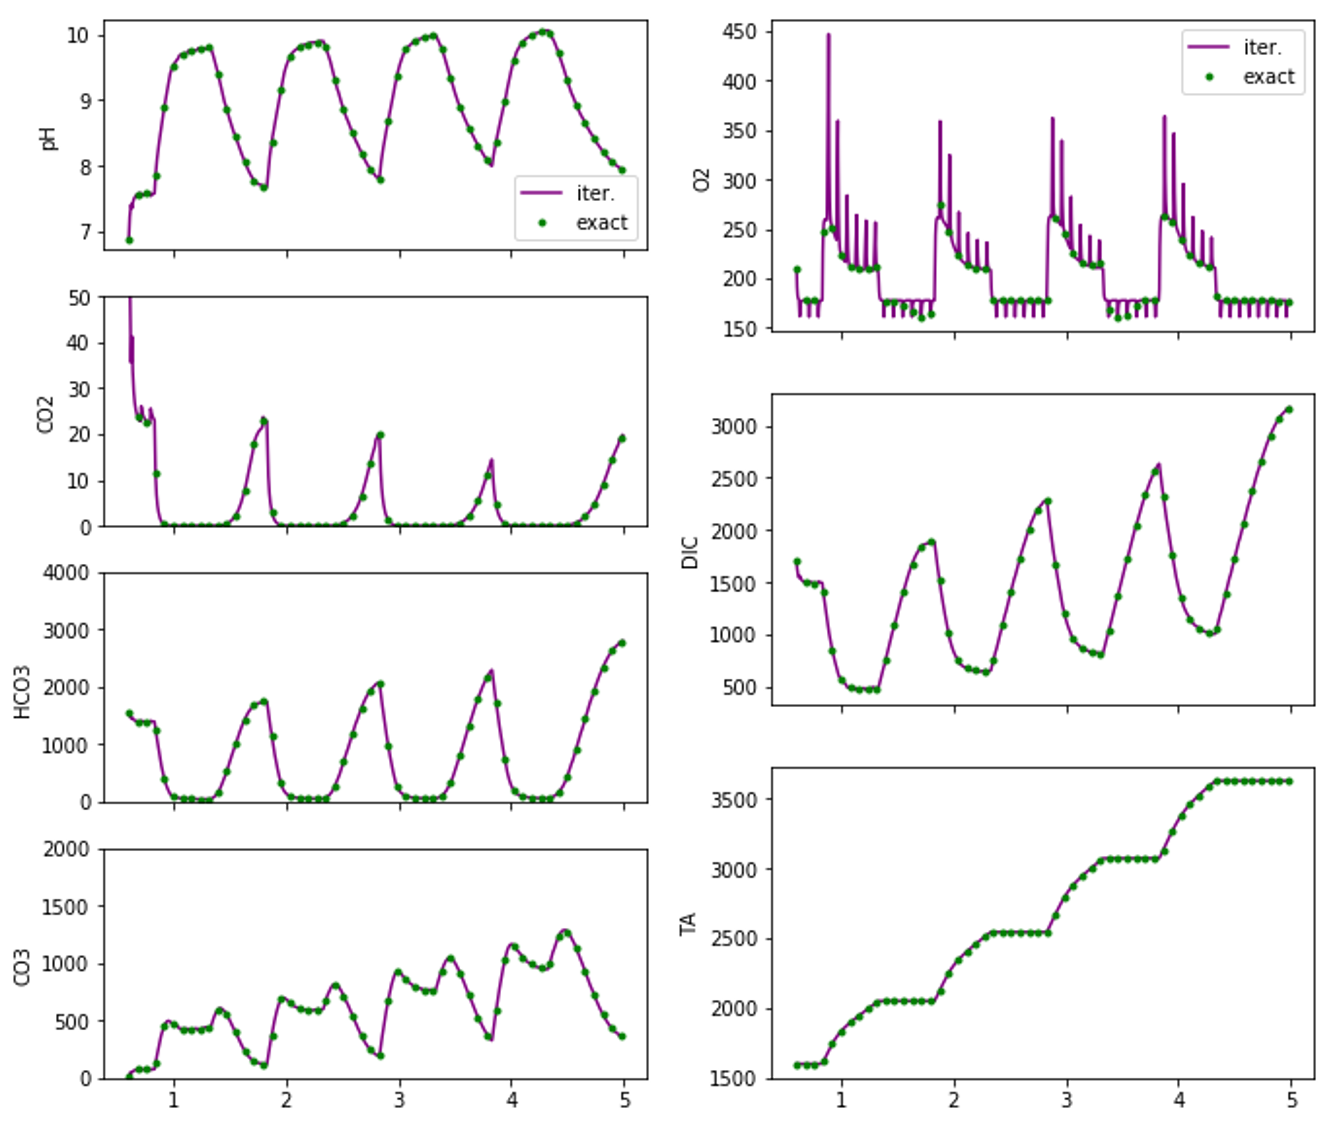
\includegraphics[width=0.9\textwidth]{images_microalgae/plots/iterative_carbon_and_states}}
	\caption[.]{Iterative (3rd iteration) vs exact solution for carbon chemistry $CO_2$, $HCO_3$, $CO_3$, $pH$ and state variables $O_2$, $DIC$, and $TA$.}
	\label{fig:iterative_carbon_and_states}
\end{figure}



\begin{table}
	\begin{tabular}{|c|c|c|c| c | c|} 
		\hline
		\bfseries{Variable} & \bfseries{Iter. 1} & \bfseries{Iter. 2} & \bfseries{Iter. 3}  &  \bfseries{Iter. 4} & \bfseries{Iter. 5} \\ \hline
		$pH$		& 0.036092734	&0.002355758	&1.41E-05		&6.93E-06		&6.93E-06 		\\
		$CO_2$		& 2.109401968	&0.145719349	&0.001222812	&0.000866728	&0.000866727 	\\
		$HCO_3$		& 19.81869214	&1.21021115		&0.008016765	&0.001025002	&0.001025139 	\\
		$CO_3$		& 20.89660704	&1.307061652	&0.00867642		&0.001102278	&0.001102434 	\\
		$DIC$		& 16.78775711	&0.958511825	&0.005229318	&0.002305054	&0.002333411 	\\
		$O_2$		&  0.308389964	&0.016044284	&4.18E-05		&6.89E-05		&7.59E-05 		\\
		$TA$		&  2.607767674	&0.160897272	&0.000688102	&0.001257725	&0.001218981 	\\
		\hline
	\end{tabular}
	\caption{RMSE for 5 iterations of the Newton-raphson carbon chemistry iterative solution.}
	\label{table:rmse_iterative}
\end{table}




%%
%% additional info
%%




%The CO2SYS Matlab version \cite{van2011matlab} was used to produce values of CO$_2$ and HCO$_3^-$ across DIC range 200-2500. 



% Total inorganic CO$_2$ (TCO$_2$) is the sum of the dissolved CO$_2$, the carbonate (CO$_{3-2}$), and the bicarbonate (HCO$_3^-$).



\FloatBarrier
\subsection{Process model: Gas transfer equilibrium concentrations for O$_2$ and CO$_2$}

%Weiss 1970 (O2) and 1974 (CO2) 

%\begin{equation}
%\begin{aligned}
%ln(Ko) =  A_{1} + A_{2}(100/T) + A_{3} ln(T/100) + S\% [B_{1} + B_{2}(T/100) + %B_{3}(T/100)^2 ] 
%\end{aligned}
%\end{equation}

The equilibrium concentration for CO$_2$ solubility in water CO$_{2H}$ ($\mu$mol/L) is calculated using Henry's law,
\begin{equation}\label{eq:CO2H_eq}
CO_{2H}=K0_{CO2}*fCO2*1.0220*1e6
\end{equation}
where fCO2 (atm) is the fugacity or approximately the partial pressure of CO$_2$, 1.0220 is the density of seawater (kg/L) at salinity 34 ppt and temperature 27$^{\circ}$C \cite{ramsing2011seawater} \cite{greensberg1992standard}. K0$_{CO2}$ (mol/kg$_{soln}$/atm) is the solubility of gas in seawater [BM: ask Chris: solubility of gas? is this right] and is calculated from the fitted van't Hoff equation and the logarithmic Setchenow salinity dependence \cite{weiss1974carbon},
\begin{equation}
\begin{aligned}
K0_{CO2} = e^{(- 60.2409 + 93.4517\frac{100}{T_K}  + 23.3585*log(\frac{T_K}{100})+ 
S(0.023517 - 0.023656\frac{T_K}{100} + 0.0047036(\frac{T_K}{100})^2))}
\end{aligned}
\end{equation}
where T$_K$ is the temperature (K) and S is salinity (ppt).
%% from Weiss 1974 paper:
%K0 may be expressed either in moles/1 * atm, referring to a liter of solution at %the temperature of the measurement and an atmosphere fugacity in
%the gas phase, or in moles/kg * atm, referring to a kilogram of solution.
Similarly the equilibrium concentration for O$_2$ solubility in water O$_{2H}$ is calculated using Henry's law,
\begin{equation}\label{eq:O2H_eq}
O_{2H}=K0_{O2}*fO2*1.0220*1e-6
\end{equation}
where fO2 (atm) is the fugacity or approximately the partial pressure of O$_2$, 1.0220 is the density of seawater (kg/L) at salinity 34 ppt and temperature 27$^{\circ}$C \cite{ramsing2011seawater} \cite{greensberg1992standard}, and K0$_{O2}$ (mol/kg$_{soln}$/atm) is the solubility of oxygen in seawater with an adjusted salinity dependence \cite{battino1983solubility},
\begin{equation}
\begin{aligned}
K0_{O2} =  \frac{e^{(-1282.8704 + \frac{36619.96}{T_K} + 223.1396 log(T_K) -0.354707 T_K 
+ S(5.957e-3 -\frac{3.7353}{T_K}) + 3.68e-6 S^2)}}{0.2094e-6}
\end{aligned}
\end{equation}
where T$_K$ is the temperature (K) and S is salinity (ppt).
%from Weiss 1970:
%\begin{equation}
%\begin{aligned}
%K0_{O2} = exp(- 58.3877 + 85.8079(100/T_K)  + 23.8439*ln(T_K/100) + \\
%S(-0.034892 + 0.015568(T_K/100) - 0.0019387(T_K/100)^2))
%\end{aligned}
%\end{equation}
The equilibrium concentrations for O$_2$ and CO$_2$ are modelled together with the gas turning on and off during the experiment, as
\begin{equation}
 Q^{air} kLa_{O_2}^{air} (O_{2H} - O_{2})
\end{equation}
\begin{equation}
 Q^{air} kLa_{CO_2}^{air} (CO_{2H} - CO_{2})
\end{equation}
where $Q^{air}$ is the gas state (1= on, 0= off), $kLa_{O_2}^{air}$ and $kLa_{CO_2}^{air}$ are the mass transfer coefficients for air (d$^{-1}$), and 0.893 is the ratio between measured $O_2$ and $CO_2$ mass transfer constants \cite{grima1993gas}.



\subsection{Process model: Photosynthesis and respiration}

Net photosynthesis
\begin{align}
\frac{\partial DIC}{dt} &=&  -(P_1 I \frac{HCO_3^-}{K_m + HCO_3^-}  - R_1) 
\\
\frac{\partial O_2}{dt}	&=&  \frac{1}{(RQ_d I + RQ_n(1-I))}(P_1 I \frac{HCO_3^-}{K_m + HCO_3^-}  - R_1)
\\
\frac{\partial TA}{\partial t}  &=&      R_R (P_1 I \frac{HCO_3^-}{K_m + HCO_3^-})
\\
\frac{\partial C_p}{\partial t} &=& (P_1 I \frac{HCO_3^-}{K_m + HCO_3^-} - R_1) 
\\\nonumber
\end{align} 
Photosynthesis ($P_1$) and respiration ($R_1$) are both modelled as random walks, by taking \begin{math}P\end{math} and \begin{math}R\end{math}, previously constant parameters, and replacing them by \begin{math}P_1(t)\end{math} and \begin{math}R_1(t)\end{math}. Here, we take \begin{math}P_1(t)\end{math} and \begin{math}R_1(t)\end{math} to be such that
\begin{displaymath}
P_1(t+\Delta t) = P_1(t) + r_P
\end{displaymath}
\begin{displaymath}
R_1(t+\Delta t) = R_1(t) + r_R
\end{displaymath}
where \begin{math}
r_P \sim N(0, \sigma_{r_P})
\end{math}, \begin{math}
r_R \sim N(0, \sigma_{r_R})
\end{math}, and \begin{math}
\Delta t
\end{math} is the length of discrete time-step. For the purpose of the Bayesian analysis here, \begin{math}\sigma_{r_P}\end{math} and \begin{math}\sigma_{r_R}\end{math} are treated as parameters to be inferred. 


$RQ_d$ and $RQ_n$ are the day and night respiratory quotients, the ratio of $CO_2$ produced and $O_2$ consumed by a cell. 




The michaelis menton term $ \frac{HCO_3^-}{K_m + HCO_3^-} $ represents the photosynthetically active carbon that the microalgae use for photosynthesis. 
%This can be CO$_2$, HCO$_3^-$, or a combination of both, eg $PAC = CO_2 + HCO_3^-$ if the microalgae are using both carbon dioxide and bicarbonate for photosynthesis.  

\subsection{Process model: Dilution}

$ \frac{Q^M}{V}(DIC^{M} - DIC) $

$ \frac{Q^M}{V}(\phantom{C}O_{2}^{M} - \phantom{CC}O_{2}) $

$ \frac{Q^M}{V}(\phantom{C}TA^{M} - \phantom{C}TA) $

$ \frac{Q^M}{V}(\phantom{CTA^{M}} - \phantom{IC}C_p) $



\subsection{Process model: Ordinary differential equations}\label{sec:micro_process_model}

A summary of the ode's that make up the process model:
\begin{align}
\text{Rate} & & \text{flux into cells}            &            &\text{gas transfer}   &     & \text{dilution} \nonumber                              \\
\frac{\partial DIC}{\partial t}&=&                      - (P_1 I \frac{HCO_3^-}{K_m + HCO_3^-} - R_1)&      &+\hat Q^{air}kLa_{ CO_2}^{air}(CO_{2}^{air} - CO_{2})                  & &+\frac{Q^M}{V}(DIC^{M} - DIC)       \nonumber \\
%                                           &  &                                   &      &+\hat Q^{co2}kLa_{ CO_2}^{co2}(CO_{2}^{co2} - CO_{2})    \\
\frac{\partial O_2}{\partial t}&=& \frac{(P_1 I \frac{HCO_3^-}{K_m + HCO_3^-} - R_1)}{(RQ_d I + RQ_n(1-I))}  &      &+\hat Q^{air}kLa_{\phantom{C}O_2}^{air}(\phantom{C}O_{2}^{air} - \phantom{I}O_{2}) && +\frac{Q^M}{V}(\phantom{C}O_{2}^{M} - \phantom{CC}O_{2})     \nonumber   \\
 %                                          &  &                                   &      &+\hat Q^{co2}kLa_{\phantom{C}O_2}^{co2}(\phantom{C}O_{2}^{co2} - \phantom{C}O_{2})    \\
\frac{\partial TA}{\partial t} & =&      R_R (P_1 I \frac{HCO_3^-}{K_m + HCO_3^-} \phantom{ + R_1})& & & & +\frac{Q^M}{V}(\phantom{C}TA^{M} - \phantom{I}TA) \nonumber\\
\frac{\partial C_p}{\partial t} & =& (P_1 I \frac{HCO_3^-}{K_m + HCO_3^-} - R_1)&  & & & +\frac{Q^M}{V}(\phantom{CTA^{M}} - \phantom{II}C_p) 
\end{align}



\begin{longtable}{|c|c|l|c|l|}
	\hline 
	& Symbol & Description  & Prior / Value & Unit \\
    \hline
    \multirow{4}{*}{\rotatebox[origin=c]{90}{Initial conditions}}
    & $DIC^0$ & Dissolved inorganic carbon & Log$\mathcal{N}$(log(1300), 0.2) & $\mu$M L$^{-1}$ \\
    & $O_2^0$ & Oxygen & Log$\mathcal{N}$(log(225), 0.2) & $\mu$M L$^{-1}$ \\
    & TA$^0$  & Total alkalinity & Log$\mathcal{N}$(log(1750), 0.1) & $\mu$M L$^{-1}$ \\
    & $C_p^0$  &  & Log$\mathcal{N}$(log(300), 0.2) & $\mu$M L$^{-1}$ \\
%    & $P^0$  & Rate of photosynthesis & & $\mu$M L$^{-1}$ day$^{-1}$\\
%    & $R^0$  & Rate of respiration & & $\mu$M L$^{-1}$ day$^{-1}$\\
    & $pH^0$ & -  & Log$\mathcal{N}$(log(8.5), 0.2) & log$_{10}$(-mol/L H+)  \\
    & $CO_2$$^0$ & Carbon dioxide  & Log$\mathcal{N}$(log(5), 0.4) & $\mu$M L$^{-1}$ \\
    & $HCO_3^-$$^0$ & Bicarbonate & Log$\mathcal{N}$(log(1500), 0.3) & $\mu$M L$^{-1}$  \\
    & $CO_3^{2-}$$^0$ & Carbonate & Log$\mathcal{N}$(log(100), 0.4) & $\mu$M L$^{-1}$ \\
    \hline
	\multirow{4}{*}{\rotatebox[origin=c]{90}{Flux into cells}}
	& $ P_1 $ & Maximum photosynthesis rate  & * & $\mu$M L$^{-1}$ hour$^{-1}$ \\
	& $ R_1 $ & Respiration rate & * & $\mu$M L$^{-1}$ hour$^{-1}$ \\ 
	& $ K_m $ & Carbon restriction & * & $\mu$M L$^{-1}$ \\
	& $ RQ_d $ & Daytime respiratory quotient & * & - \\
	& $ RQ_n $ & Night respiratory quotient & * & - \\
	& $ R_R $ & Redfield ratio & * & - \\
	& $ I $ & Light indicator & forcing (0/1) & - \\	
    \hline
    \multirow{4}{*}{\rotatebox[origin=c]{90}{Gas transfer terms }}
    & $ \hat Q ^{air} $ & Indicator for flow in air line  & forcing (0/1) & - \\
    & $x_{CO_2}^{air} $ & Mole fraction of CO$_2$ atmosphere & 400 & ppm \\ 
    & $CO_{2H}$  & Equilibrium CO$_2$ concentration  & Eq. \ref{eq:CO2H_eq} & $\mu$M L$^{-1}$  \\
    & $CO_{2}^{air}$ & Sat CO$_2$ conc with atmosphere &   $x_{CO_2}^{air} CO_{2H}$ & \\
    & $kLa_{ CO_2}^{air}$ & Mass transfer coefficient for CO$_2$ & 0.893$kLa_{\phantom{C}O_2}^{air}$  & day$^{-1}$ \\
    
    & $x_{O_2}^{air} $ & Mole fraction of O$_2$ atmosphere& 0.2094 & atm \\ 
    & $\phantom{C}O_{2H}$  & Equilibrium O$_2$ concentration  & Eq. \ref{eq:O2H_eq} & $\mu$M L$^{-1}$  \\
	& $\phantom{C}O_{2}^{air}$ & Sat O$_2$ conc with atmosphere &   $x_{O_2}^{air} O_{2H}$ & \\
    & $\tau$ & half-life of $kLa_{\phantom{C}O_2}^{air}$  & range(2-20) & min$^{-1}$\\
    & $kLa_{\phantom{C}O_2}^{air}$ & Mass transfer coefficient for O$_2$ & $\ln(2) * 24*60/\tau$ & day$^{-1}$\\
   
    \hline
        \multirow{4}{*}{\rotatebox[origin=c]{90}{Dilution terms }}
    &$  Q ^{M} $ & Dilution rate  & forcing & ml day$^{-1}$ \\
    &$  V $ & Volume of the reactor  & 500 & ml \\
    &$  DIC ^{M} $ & Media dissolved inorganic carbon  & 1724.20 & $\mu$M L$^{-1}$ \\ 
    &$	\phantom{CC}O_2^{M}$ & Media oxygen concentration & 226.65 & $\mu$M L$^{-1}$ \\
    &$	\phantom{C}TA^{M}$  & Media total alkalinity & 1797.90 & $\mu$M L$^{-1}$
    \\
    
        \hline
%    \multirow{4}{*}{\rotatebox[origin=c]{90}{Other dilution terms }}
%    &$ \hat Q ^{CO2} $ &indicator for dilution & 0 or 1 & - \\
%  
%    & $x_{\phantom{C}O_2}^{CO2} $ & mole fraction of & 0 & - \\ 
%    & $\phantom{C}O_{2}^{CO2}$ & sat CO$_2$ conc with CO$_2$ &   $x_{O_2}^{CO2} O_{2H}$ & \\
%    & $kLa_{ \phantom{C}O_2}^{CO2}$ & mass transfer coefficient &   & day$^{-1}$ \\
%    & $\phantom{C}O_2^{CO2}$  & & & \\
%    
%    & $x_{CO_2}^{CO2} $ & mole fraction of  & 1 & ppm \\ 
%    & $CO_{2}^{CO2}$ & sat CO$_2$ conc with CO$_2$ &   $x_{CO_2}^{CO2} CO_{2H}$ & \\
%    & $kLa_{ CO_2}^{CO2}$ & mass transfer coefficient & 0.893$kLa_{\phantom{C}O_2}^{CO2}$  & day$^{-1}$ \\
%    &$  CO_{2} ^{CO2} $ &   &  &  \\   
%    \hline
	\caption{State variable, parameter and forcing definitions with units, and their assignments: either fixed values, priors on initial condition or priors on parameters (*) defined later in Section \ref{sec:micro_parameter_model}.}
\end{longtable}  
    



%\clearpage
%\begin{tabular}{l l  | l}
%	 \hline 
%	Symbol & Variable & Units  \\ \hline
%	DIC &  Dissolved inorganic carbon concentration & $\mu$mol/L  \\
%	O$_2$ & Oxygen  &  $\mu$mol/L \\
%	pH & -  & log$_{10}$(-mol/L H+)  \\
%	CO$_2$ & Carbon dioxide  & $\mu$mol/L \\
%	HCO$_3^-$ & Bicarbonate & $\mu$mol/L  \\
%	CO$_3^{2-}$ & Carbonate  & $\mu$mol/L \\
%	kLA$_{O2}$  & Mass transfer coefficient for O$_2$ &  d$^{-1}$  \\
%	
%	CO$_{2H}$  & Equilibrium CO$_2$ concentration  & $\mu$mols/L  \\
%	
%	K0$_{O2}$ &  Solubility of gas & mol/kg$_{soln}$/atm  \\
%	K0$_{CO2}$ & Solubility of gas & mol/kg$_{soln}$/atm   \\
%	TA  & Total alkalinity & $\mu$mols/L  \\
%	S  & Salinity &  ppt  \\
%	fCO2  & Fugacity/CO$_2$ partial pressure &  atm  \\
%	fO2  & Fugacity/O$_2$ partial pressure &  atm \\
%	
%	K$_m$ & Carbon restriction & $\mu$mols/L \\
%	
%	P & Photosynthesis rate & $\mu$mols/L/day \\
%	R & Respiration rate & $\mu$mols/L/day \\
%	R$_R$ & Redfield ratio & - \\	
%	R$_Q$ & Respiratory quotient & - \\
%\end{tabular}
%\captionof{table}{Table of variables and parameters.}

%\begin{tabular}{c c  | c}
%	 \hline
%	 Symbol & Variable & Units  \\ \hline
%	I &  Light Intensity  &  normalised to 0/1   \\
%	T & Temperature & $\circ$ C  \\
%	T$_K$ & Temperature &  K  \\
%	$\xi$ & gasflow &  on/off (1,0)  \\
%	
%\end{tabular}
%\captionof{table}{Table of Forcings}


\subsection{Design and setup of data assimilation model with both simulated and experimental data}

A simulated dataset was created by running the process model described in Section \ref{sec:micro_process_model} with a fixed set of parameters ($P_1$ = 200, $R_1$ = 30, $kLA_{O_2}^{air}$ = 200, $K_m$ = 150, $RQ_d$ = 0.85, $RQ_n$ = 0.95, $R_R$ = 0.075) and initial conditions ($O_2^0$ = 225, $DIC^0$ = 1250, $TA^0$ = 1750). 

The first set of results will assimilate the simulated observations and attempt to recover the true value parameters. 

[Chris: noise on simulated dataset? sigmas? can you double check what I've written here is right?]

\subsection{Parameter Model: Priors} \label{sec:micro_parameter_model}
** include simulated data priors, and real data priors.

Decide whether the parameters vary in time or not.




\begin{tabular}{c | c  |  c}
	Parameter & Prior &  Proposal \\ \hline
	S  & 34 & * \\
	fCO2  & 397e-6 &  *  \\
	fO2  & 0.21 &  *  \\
	kLA$_{O2}$  & LogNormal(log(200.0), 0.5)  & LogNormal(log(kLA$_{O2}$), 0.5prop$_{std}$) \\
	K$_m$ &  LogNormal(log(200.0), 0.8)  & LogNormal(log(K$_m$), 0.8prop$_{std}$) \\
	R$_R$  & Uniform(0.0001, 0.2) &  TrunNormal(R$_R$, 0.2prop$_{std}$, 0.0001, 0.2) \\
	R$_Q$  & Uniform(0.66, 1) &  TrunNormal(R$_Q$, 0.2prop$_{std}$, 0.66, 1.0)
	 \\
	$\sigma_P$ & Normal(0.05, 0.01) & Normal($\sigma_P$, 0.01prop$_{std}$) \\
	$\sigma_R$ & Normal(0.01, 0.001) & Normal($\sigma_R$, 0.001prop$_{std}$) \\
	
%R$_1$ & LogNormal(log(1000.0), 0.3)  & LogNormal(log(R$_1$), 0.3prop$_{std}$) \\	
%	P$_1$ & 4.7407e-4 $\pm$ & - \\
\end{tabular}
\captionof{table}{Table of Parameters, their priors and proposal distributions. * indicates the parameter was held fixed. (prop$_{std}$ =0.1)}
\newpage


\FloatBarrier

\section{Results and Discussion}



%% for reference
%Approximating equations in place of CO2SYS:
%
%\begin{equation}
%\begin{aligned}
%HCO_3^- = exp(16.262 + 0.0047081*DIC - 0.11922*T + 0.0050303*alk1 \\
%+ 1.7093*log(DIC) + 0.38048*log(S) - 3.7548*log(alk1)\\
%- 2.292e-5*DIC*T - 0.0032028*DIC*log(DIC) - 0.00015313*DIC*log(S)\\
%+ 0.0032527*DIC*log(alk1) +\\ 0.021965*T*log(alk1) - 0.00090344*alk1*log(DIC))
%\end{aligned}
%\end{equation}
%
%\begin{equation}
%\begin{aligned}
%CO_2 = exp(-486.84 - 0.070754*DIC - 0.25277*T - 0.20674*S - \\
%0.11627*alk1 + 78.274*log(DIC) + 72.147*log(alk1) - 2.9438e-5*DIC*T\\
% - 5.8841e-6*DIC*alk1 - 0.0040234*DIC*log(DIC) + 0.016172*DIC*log(alk1)\\
% - 0.02039*T*log(DIC) + 0.062452*T*log(alk1) + 0.029857*S*log(alk1) \\
% + 0.0031507*alk1*log(DIC) + 0.010398*alk1*log(alk1) \\
% - 11.192*log(DIC)*log(alk1))
%\end{aligned}
%\end{equation}
%
%\begin{equation}
%\begin{aligned}
%pH = 9.5803 - 0.0027089*DIC - 0.018089*T - 0.012068*S + 0.0016329*alk1\\
%+ 1.2706e-5*DIC*T + 4.6961e-7*DIC*alk1 - 9.2122e-6*T*alk1 - \\
%5.9777e-8*DIC**2 - 2.194e-7*alk1**2 
%\end{aligned}
%\end{equation}



%% For reference

%\begin{equation}
%HCO_3^- =  -818.0204 +   1.9388 DIC  +  0.0681alk  -0.0003 DIC alk
%\end{equation}
%
%\begin{equation}
%\begin{aligned}
%CO_2 = exp(-10.6788 +   0.0096 DIC +   0.1479 T +   0.0330 S  -0.0015 alk \\
%-6.2777e-05 DIC T   - 8.778e-07 DIC alk)
%\end{aligned}
%\end{equation}
%
%\begin{equation}
%\begin{aligned}
%pH = 12.26 -0.0030605 DIC -0.043752 T -0.013625 S+ 0.00011315 alk\\
%+ 1.3463e-05 DIC T + 5.2215e-07 DIC alk
%\end{aligned}
%\end{equation}


\FloatBarrier
\subsection{Posteriors with simulated data}


\begin{figure}
	\centerline{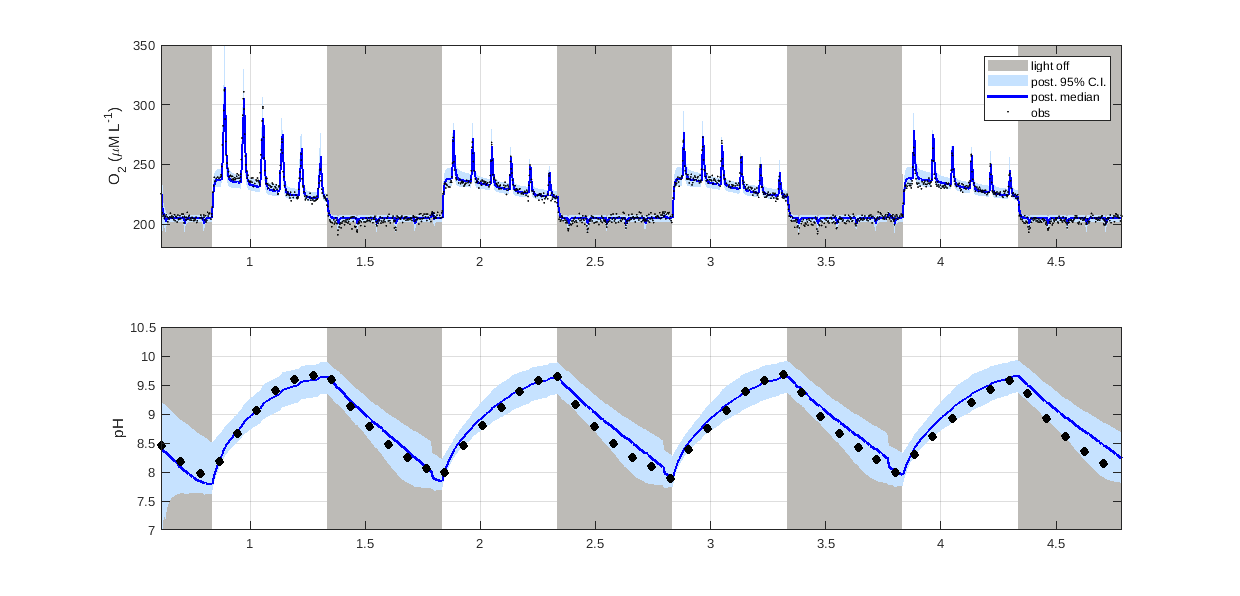
\includegraphics[width=1.2\textwidth]{images_microalgae/posterior_plots_with_fake_data/O2_pH}}
	\caption[.]{Posterior medians (solid blue line), 95\% credible intervals (shaded blue), and simulated observations (black) for $O_2$ and $pH$ across 4 days.}
	\label{fig:pos_sim_O2_pH}
\end{figure}

\begin{figure}
	\centerline{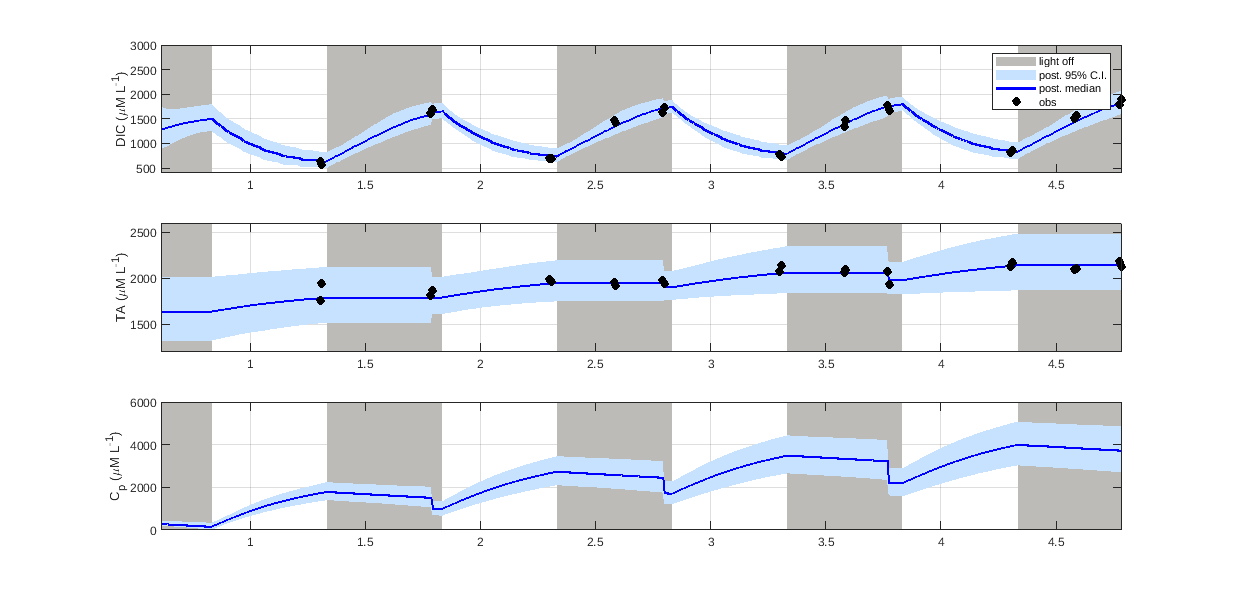
\includegraphics[width=1.2\textwidth]{images_microalgae/posterior_plots_with_fake_data/DIC_TA_Cp}}
	\caption[.]{Posterior medians (solid blue line), 95\% credible intervals (shaded blue), and simulated observations (black) for $DIC$, $TA$ and $C_p$ across 4 days.}
	\label{fig:pos_sim_DIC_TA_Cp}
\end{figure}

\begin{figure}
	\centerline{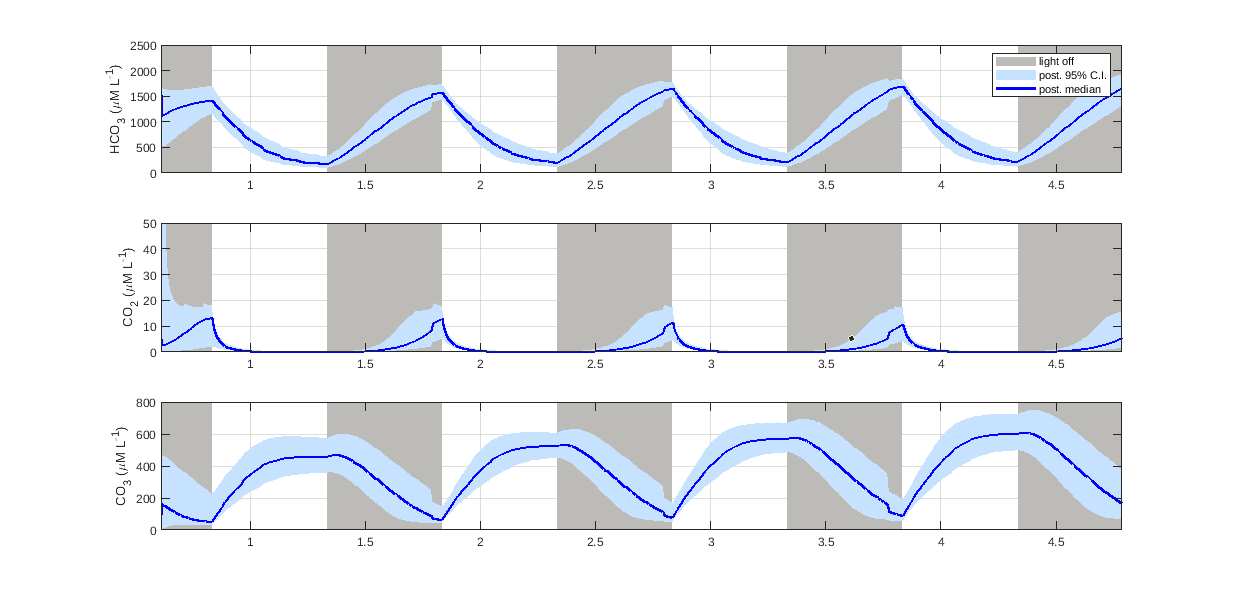
\includegraphics[width=1.2\textwidth]{images_microalgae/posterior_plots_with_fake_data/carbon}}
	\caption[.]{Posterior medians (solid blue line) and 95\% credible intervals (shaded blue) for $HCO_3$, $CO_2$ and $CO_3$ across 4 days.}
	\label{fig:pos_sim_carbon}
\end{figure}


\begin{figure}
	\centerline{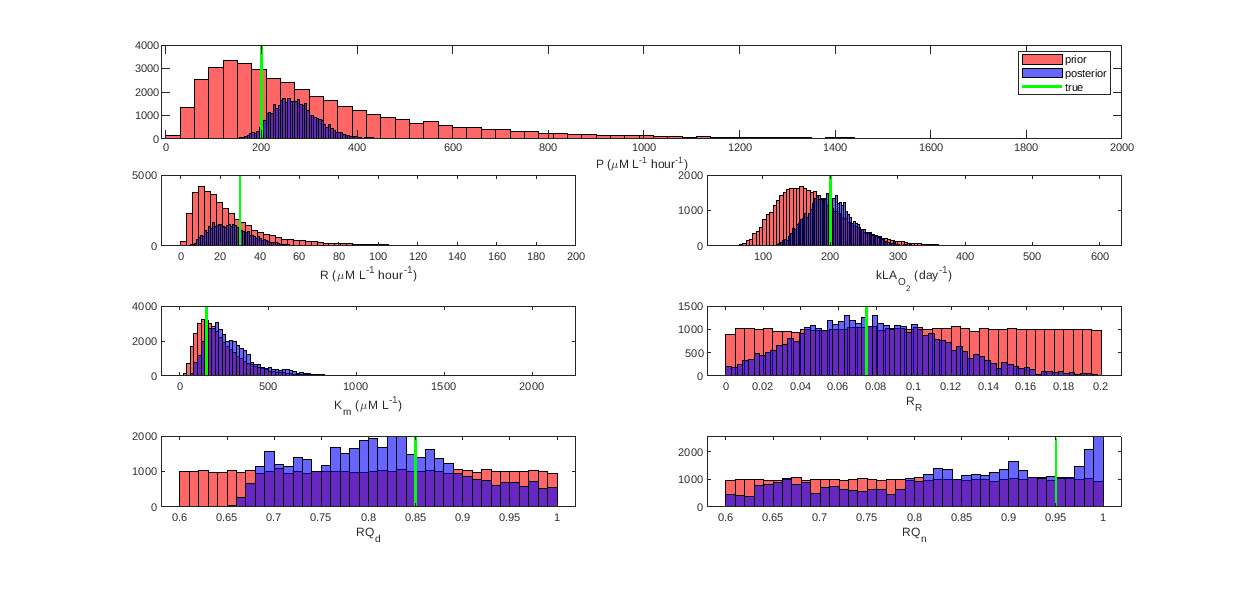
\includegraphics[width=1.3\textwidth]{images_microalgae/posterior_plots_with_fake_data/model_parameters}}
	\caption[.]{Priors (pink), posteriors (purple) and true values (green) for model parameters.}
	\label{fig:pos_sim_model_parameters}
\end{figure}


\begin{longtable}{|c|c|c|c|} 
		\hline
		\bfseries{Parameter}  & \bfseries{Quantiles (25\%, 75\%)}  & \bfseries{Quantiles (5\%, 95\%)} &  \bfseries{True value} \\ \hline
		$P_1$ 				& (237.2167, 302.0565) 	& (200.8971, 365.1751) 	&  200  \\ 
		$R_1$ 				& (17.5370, 32.3501) 	& (10.6537, 45.3096)	& 	30 \\ 
		$kLA_{O_2}^{air}$ 	& (177.1383, 222.9641)  & (148.2838, 267.5934)  &  200 \\
		$K_m$ 				& (182.6643, 362.6714) 	& (118.4125, 643.8518) 	&  150 \\ 
		$R_R$ 				& (0.0504, 0.1041) 		& (0.0196, 0.1458) 		& 0.075 \\
		$RQ_d$ 				& (0.7529, 0.8718) 		& (0.6894, 0.9666) 		& 0.85 \\	
		$RQ_n$ 				& (0.7469, 0.9338) 		& (0.6400, 0.9920) 		& 0.95 \\	
		\hline
		\caption[.]{True values for parameters used to create the simulated observations, and posterior (25\%, 75\%), (5\%, 95\%) quantiles for parameters after assimilating observations.}	
		\label{table:micro_parameters_sim}
\end{longtable}

After 50,000 samples the true values of parameters $R_1$, $kLA_{O_2}^{air}$, $R_R$, and $RQ_d$ were recovered to the 25th and 75th percentile (Table \ref{table:micro_parameters_sim}). While the true values of $K_m$ and $RQ_n$ did not lie within the 25th and 75th quantile, they were captured by the 5th and 95th percentiles (Table \ref{table:micro_parameters_sim}). $P_1$ was the only parameter whose true value lied on the cusp of the 5th percentile. Parameters $P_1$, $R_1$, $kLA_{O_2}^{air}$, and $R_R$ mixed well, while parameters $K_m$, $RQ_d$, and $RQ_n$ did not mix as well, some autocorrelation between samples was present (Figure \ref{fig:micro_sim_model_parameters_traces}).


Log-likelihood stopped rising (Figure \ref{fig:micro_sim_loglikelihood}).
Acceptance rate was XX.


Observed state variables $O_2$, $DIC$, $TA$, and observed $pH$ posteriors were in excellent agreement with observations, with all observations fitting within the 95\% credible interval posteriors (Figure \ref{fig:pos_sim_O2_pH}, Figure \ref{fig:pos_sim_DIC_TA_Cp}).

Unobserved state variable $C_p$ .. (Figure \ref{fig:pos_sim_DIC_TA_Cp}).

Carbon chemistry variables $HCO_3$, $CO_2$, and $CO_3$ ... (Figure \ref{fig:pos_sim_carbon}).


\FloatBarrier
\subsection{Posteriors with simulated data version 2}


\begin{figure}
	\centerline{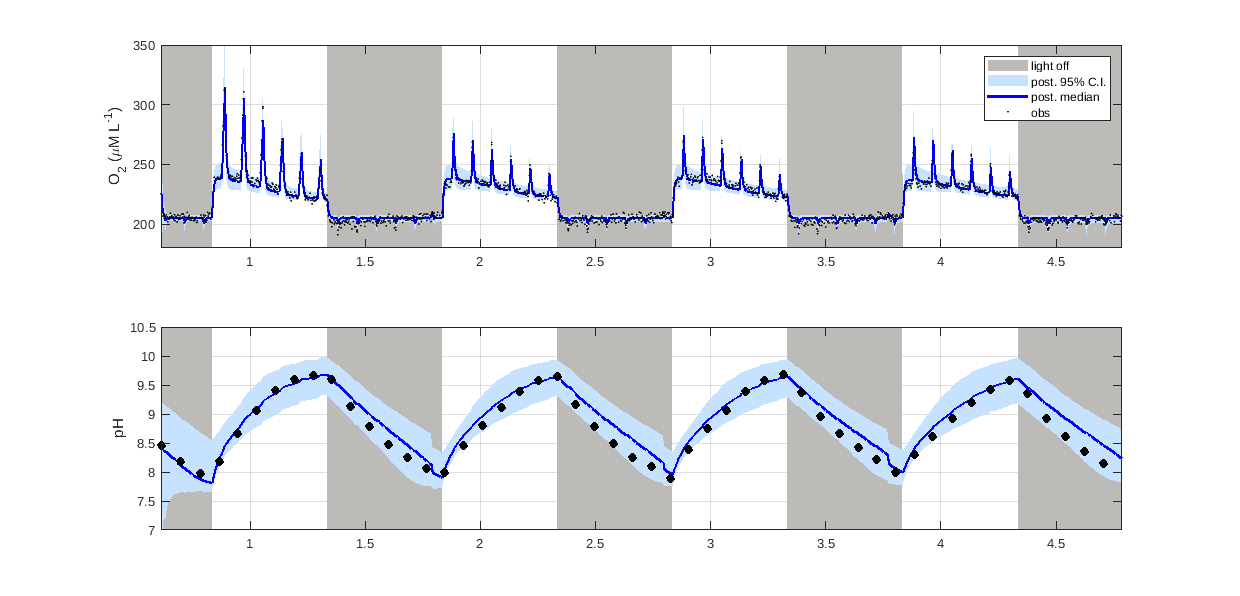
\includegraphics[width=1.2\textwidth]{images_microalgae/posterior_plots_with_fake_data_other/O2_pH}}
	\caption[.]{Posterior medians (solid blue line), 95\% credible intervals (shaded blue), and simulated observations (black) for $O_2$ and $pH$ across 4 days.}
	\label{fig:pos_sim_O2_pH_other}
\end{figure}

\begin{figure}
	\centerline{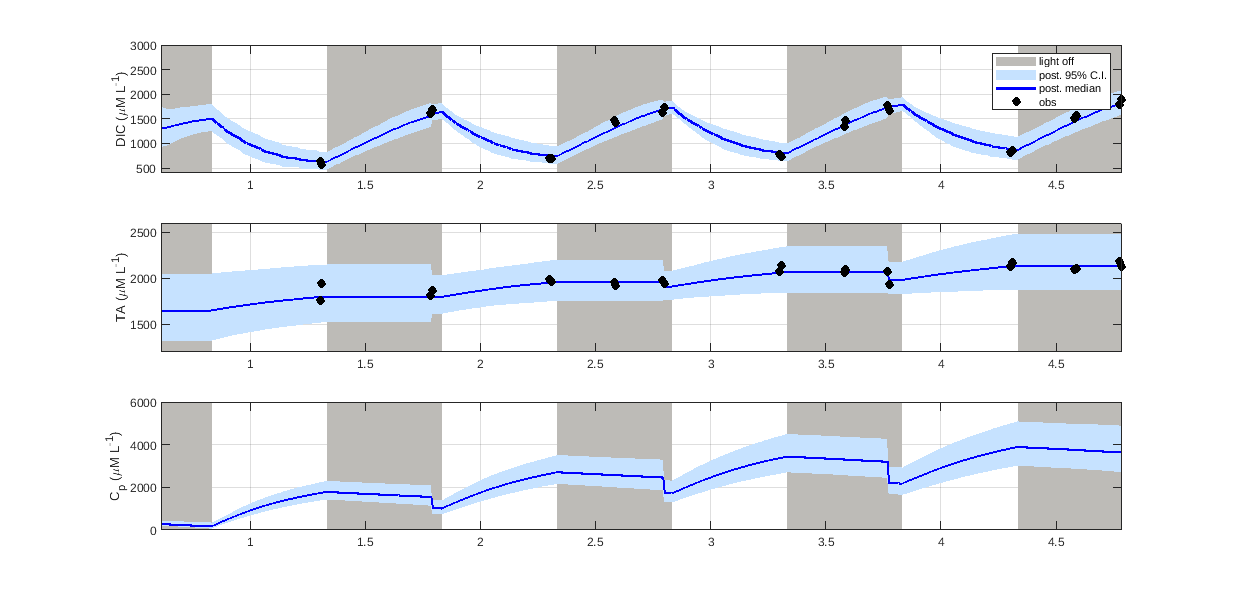
\includegraphics[width=1.2\textwidth]{images_microalgae/posterior_plots_with_fake_data_other/DIC_TA_Cp}}
	\caption[.]{Posterior medians (solid blue line), 95\% credible intervals (shaded blue), and simulated observations (black) for $DIC$, $TA$ and $C_p$ across 4 days.}
	\label{fig:pos_sim_DIC_TA_Cp_other}
\end{figure}

\begin{figure}
	\centerline{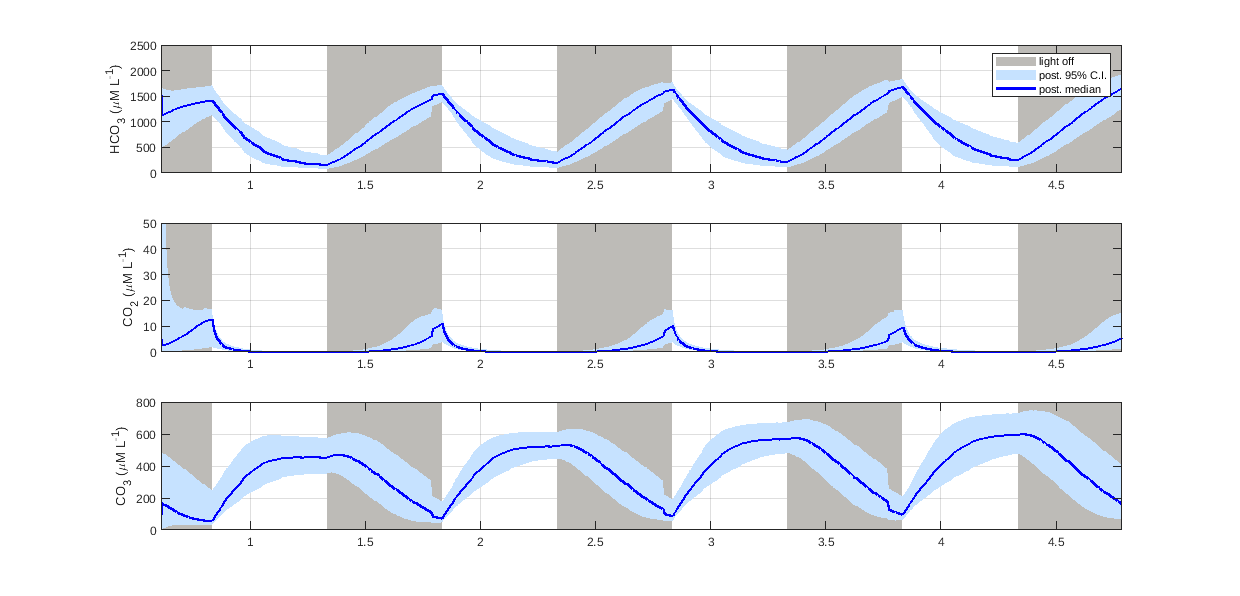
\includegraphics[width=1.2\textwidth]{images_microalgae/posterior_plots_with_fake_data_other/carbon}}
	\caption[.]{Posterior medians (solid blue line) and 95\% credible intervals (shaded blue) for $HCO_3$, $CO_2$ and $CO_3$ across 4 days.}
	\label{fig:pos_sim_carbon_other}
\end{figure}


\begin{figure}
	\centerline{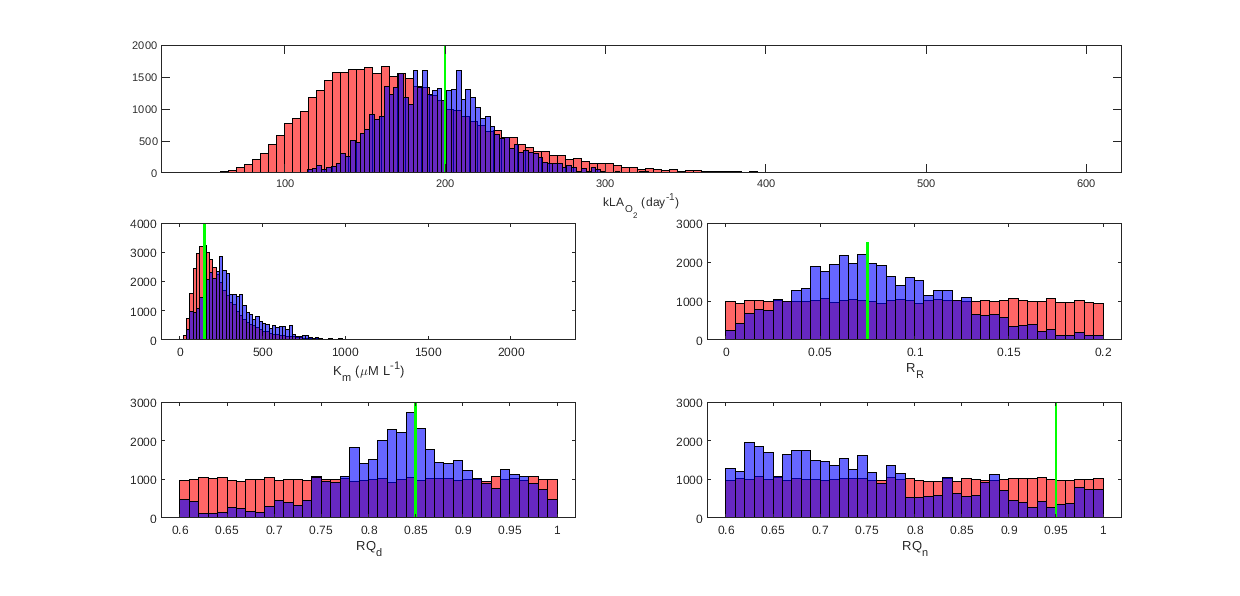
\includegraphics[width=1.3\textwidth]{images_microalgae/posterior_plots_with_fake_data_other/model_parameters}}
	\caption[.]{Priors (pink), posteriors (purple) and true values (green) for model parameters.}
	\label{fig:pos_sim_model_parameters_other}
\end{figure}

\begin{figure}
	\centerline{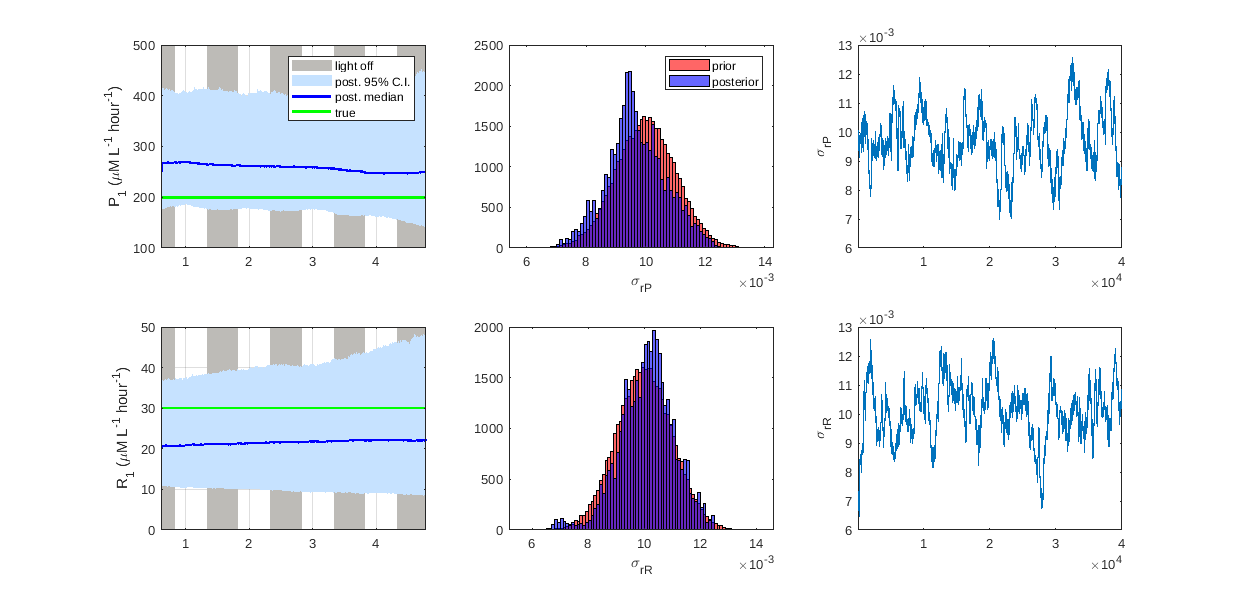
\includegraphics[width=1.3\textwidth]{images_microalgae/posterior_plots_with_fake_data_other/P_and_R}}
	\caption[.]{Random walk posteriors $P_1$ and $R_1$ medians (solid blue), 95\% credible intervals (shaded blue), and true values (green). $\sigma_{rP}$ and $\sigma_{rR}$ priors (pink), posteriors (purple), true values (green) and traces.}
	\label{fig:pos_sim_P_and_R_other}
\end{figure}

\begin{figure}
	\centerline{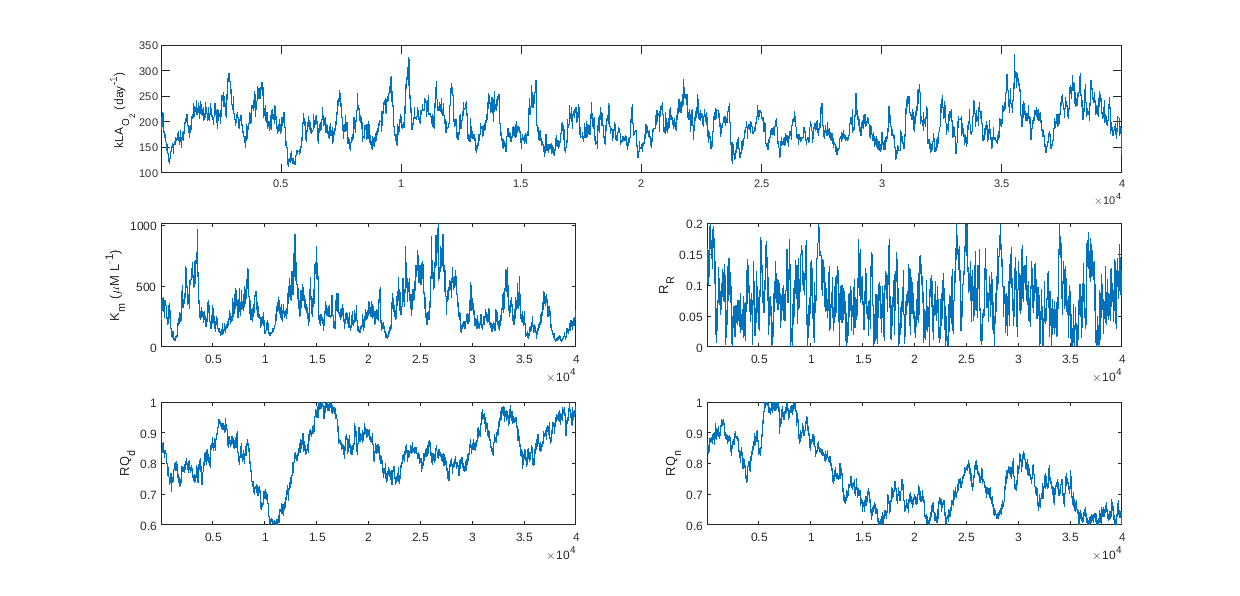
\includegraphics[width=1.3\textwidth]{images_microalgae/posterior_plots_with_fake_data_other/model_parameters_traces}}
	\caption[.]{Traces for model parameters.}
	\label{fig:micro_sim_model_parameters_other_trace}
\end{figure}

\begin{longtable}{|c|c|c|c|} 
	\hline
	\bfseries{Parameter}  & \bfseries{Quantiles (25\%, 75\%)}  & \bfseries{Quantiles (5\%, 95\%)} &  \bfseries{True value} \\ \hline
	$P_1$ 				& () 					& () 					&  200  \\ 
	$R_1$ 				& () 					& ()					& 	30 \\ 
	$kLA_{O_2}^{air}$ 	& (170.9854, 216.0578)  & (145.6899, 253.4652)  &  200 \\
	$K_m$ 				& (187.3586, 386.4103) 	& (93.9670, 641.1432) 	&  150 \\ 
	$R_R$ 				& (0.0521, 0.1075) 		& (0.0192, 0.1544) 		& 0.075 \\
	$RQ_d$ 				& (0.7906, 0.8965) 		& (0.6833, 0.9711) 		& 0.85 \\	
	$RQ_n$ 				& (0.6654, 0.8334) 		& (0.6164, 0.9739) 		& 0.95 \\	
	\hline
	\caption[.]{True values for parameters used to create the simulated observations, and posterior (25\%, 75\%), (5\%, 95\%) quantiles for parameters after assimilating observations.}	
	\label{table:micro_parameters_sim_other}
\end{longtable}

Ran for 50,000 samples, discarded first 10,000 as burn-in. $P_1$ and $R_1$ as random walks with $\sigma_{rP}$ and $\sigma_{rR}$ as standard deviations of the random walks and parameters to be estimated.  

After 50,000 samples the true values of parameters $kLA_{O_2}^{air}$, $R_R$, and $RQ_d$ were recovered to the 25th and 75th percentile (Table \ref{table:micro_parameters_sim_other}). While the true values of $K_m$ and $RQ_n$ did not lie within the 25th and 75th quantile, they were captured by the 5th and 95th percentiles (Table \ref{table:micro_parameters_sim_other}). 
Parameters $\sigma_{rP}$, $\sigma_{rR}$, $kLA_{O_2}^{air}$, and $R_R$ mixed well, while parameters $K_m$, $RQ_d$, and $RQ_n$ did not mix as well, some autocorrelation between samples was present (Figure \ref{fig:micro_sim_model_parameters_other_trace}).

****This results section came out the same as the first model with the simulated observations.

\FloatBarrier
\subsection{Posteriors with experimental data}

40,000 samples run with 1024 particles (40,000 was all that could complete in the maximum time allocation on the hpc cluster). 10,000 discarded as burn-in, acceptance rate was XX.

$P_1$ and $R_1$ are random walks. $RQ_d$ and $RQ_n$ are random walks. State posteriors are visualised by plotting the median and shading 95\% credible intervals, while parameter priors and posteriors are displayed by histograms.

\begin{figure}
	\centerline{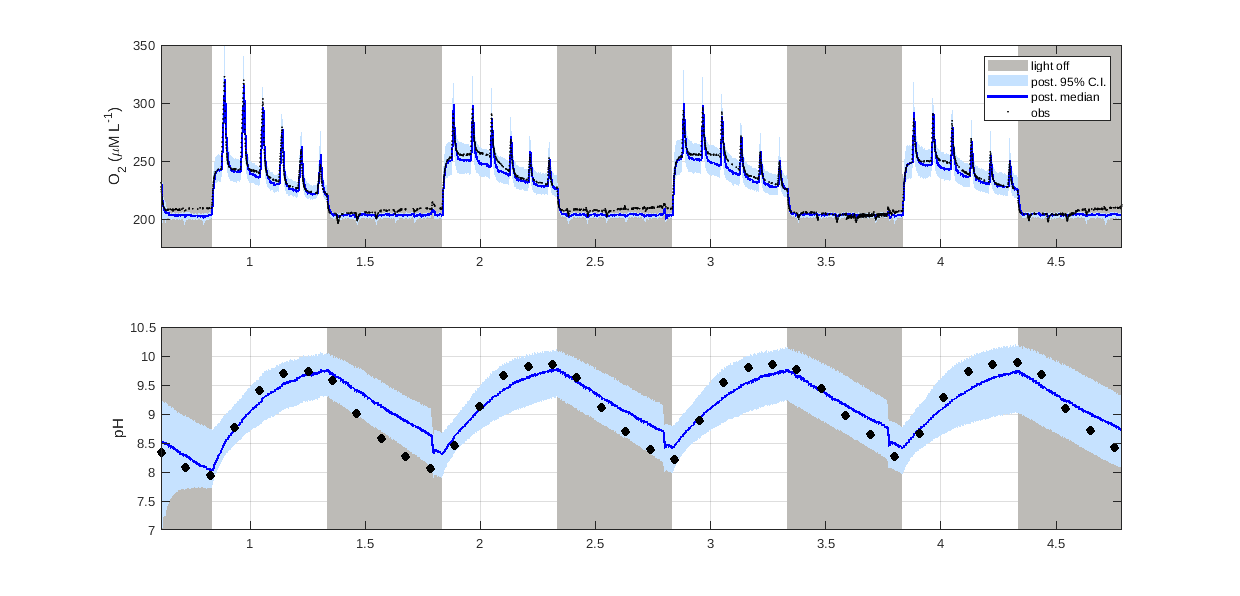
\includegraphics[width=1.2\textwidth]{images_microalgae/plots_chris/O2_pH}}
	\caption[.]{Posterior medians (solid blue line), 95\% credible intervals (shaded blue), and simulated observations (black) for $O_2$ and $pH$ across 4 days.}
	\label{fig:pos_O2_pH}
\end{figure}

\begin{figure}
	\centerline{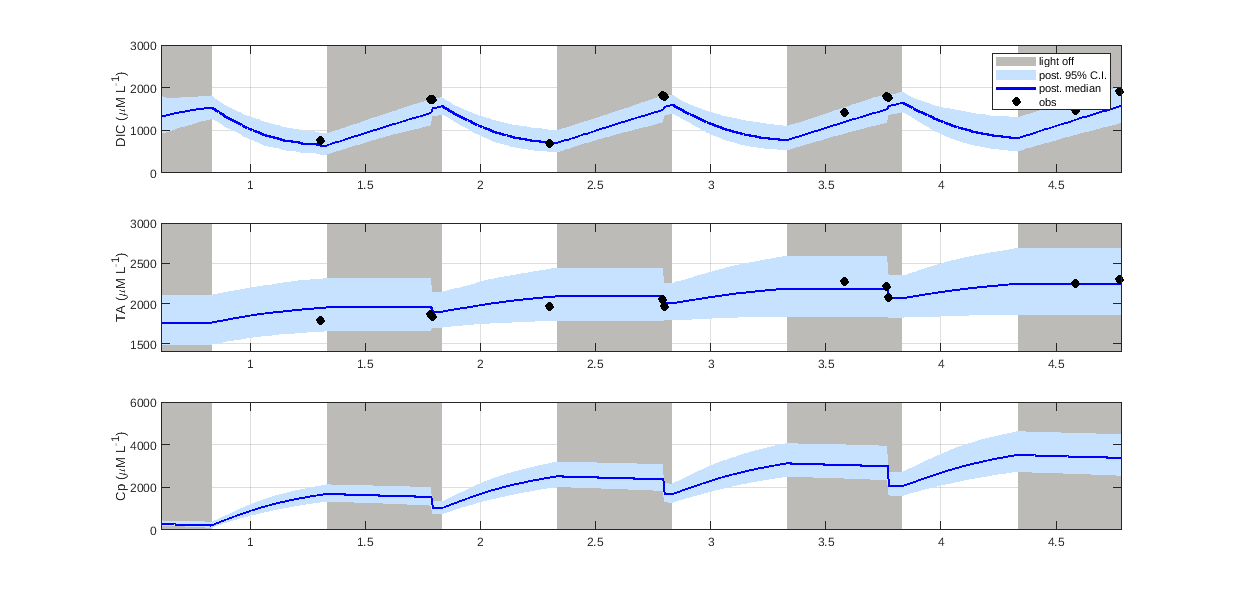
\includegraphics[width=1.2\textwidth]{images_microalgae/plots_chris/DIC_TA_Cp}}
	\caption[.]{Posterior medians (solid blue line), 95\% credible intervals (shaded blue), and simulated observations (black) for $DIC$, $TA$ and $C_p$ across 4 days.}
	\label{fig:pos_DIC_TA}
\end{figure}

\begin{figure}
	\centerline{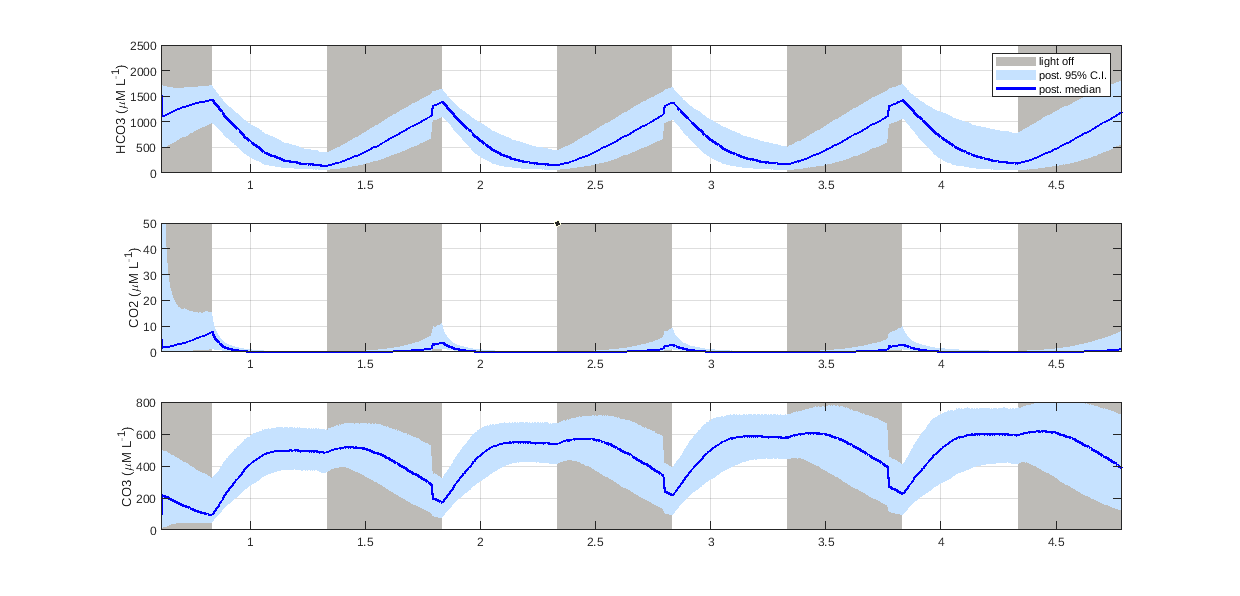
\includegraphics[width=1.2\textwidth]{images_microalgae/plots_chris/carbon}}
	\caption[.]{Posterior medians (solid blue line) and 95\% credible intervals (shaded blue) for $HCO_3$, $CO_2$ and $CO_3$ across 4 days.}
	\label{fig:pos_carbon}
\end{figure}

\begin{figure}
	\centerline{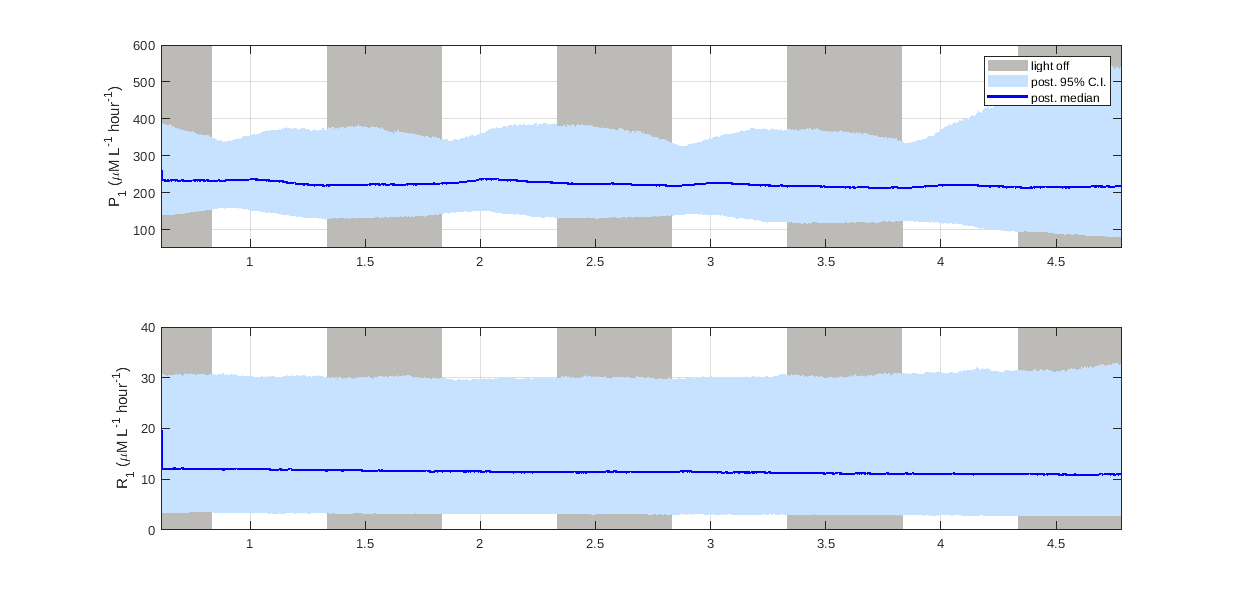
\includegraphics[width=1.2\textwidth]{images_microalgae/plots_chris/P_and_R}}
	\caption[.]{Posterior medians (solid blue line) and 95\% credible intervals (shaded blue) for photosynthesis $P_1$ and respiration $R_1$.}
	\label{fig:pos_P_R}
\end{figure}

\begin{figure}
	\centerline{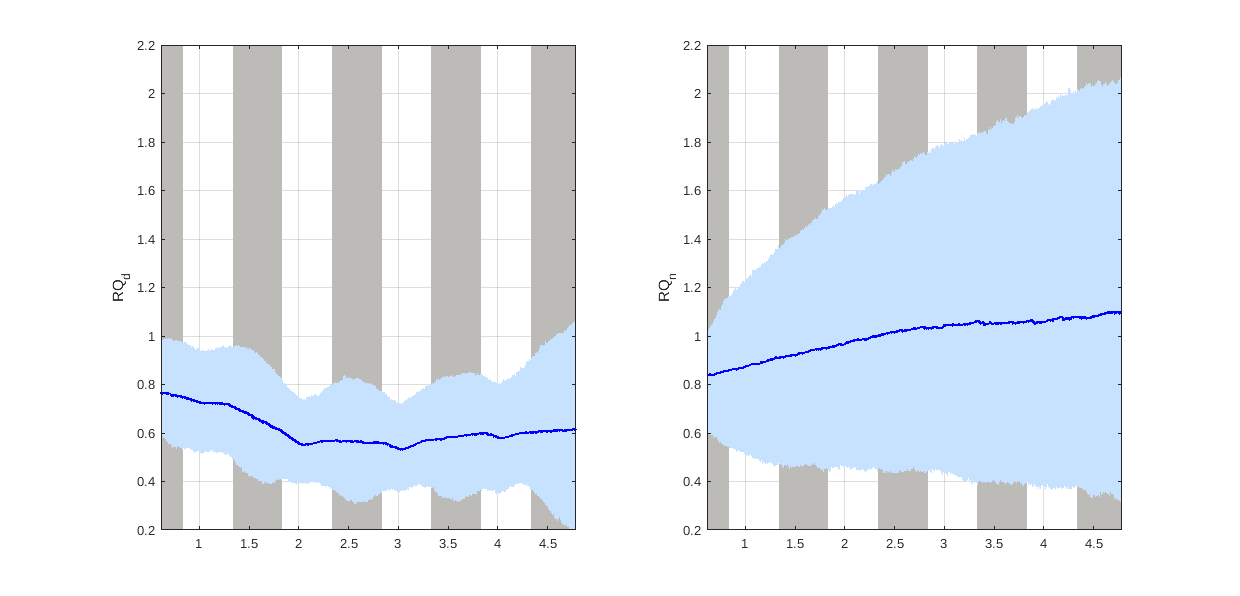
\includegraphics[width=1.2\textwidth]{images_microalgae/plots_chris/RQ_d_RQ_n}}
	\caption[.]{Posterior medians (solid blue line) and 95\% credible intervals (shaded blue) for $RQ_d$ and $RQ_n$.}
	\label{fig:pos_RQ_d_RQ_n}
\end{figure}



\begin{figure}
	\centerline{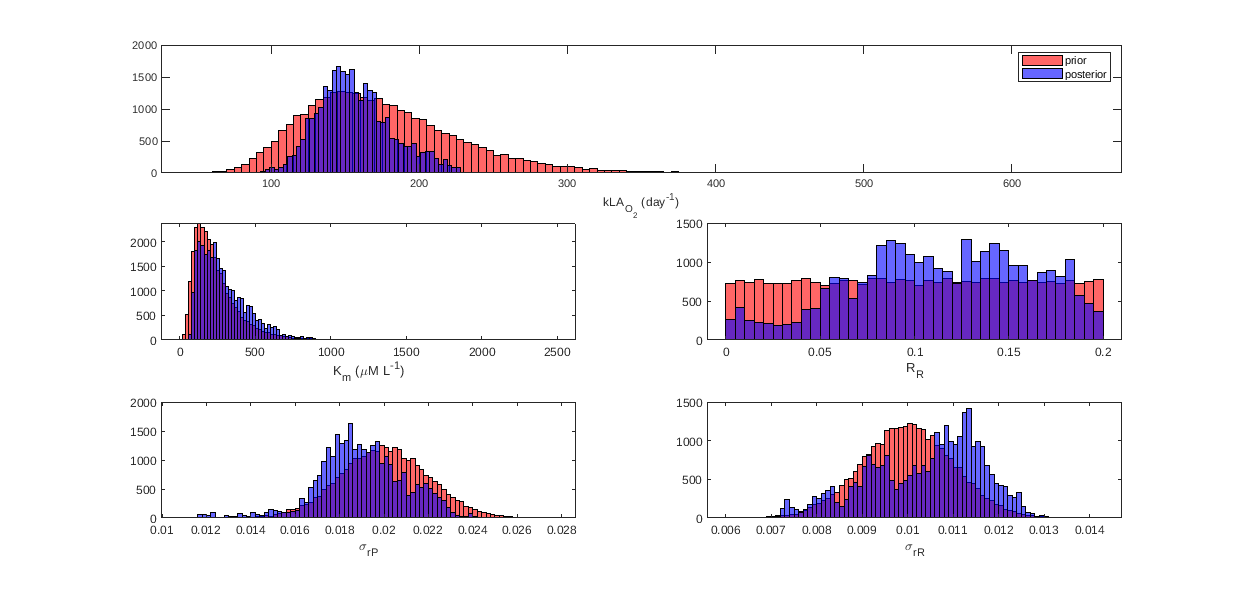
\includegraphics[width=1.3\textwidth]{images_microalgae/plots_chris/modelparameters1}}
	\caption[.]{Priors (pink) and posteriors (purple) for model parameters.}
	\label{fig:pos_parameters_model}
\end{figure}

\begin{figure}
	\centerline{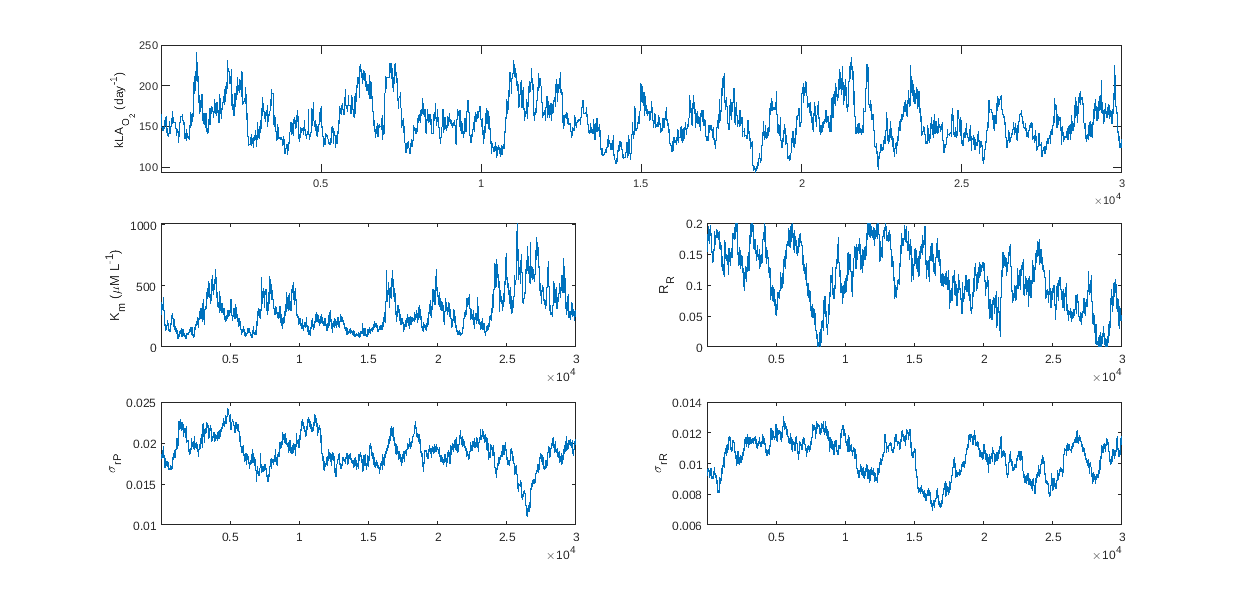
\includegraphics[width=1.3\textwidth]{images_microalgae/plots_chris/modelparameters1_trace}}
	\caption[.]{Traces for model parameters.}
	\label{fig:pos_parameters_model2}
\end{figure}



\begin{longtable}{|c|c|c|} 
	\hline
	\bfseries{Parameter}  & \bfseries{Quantiles (25\%, 75\%)}  & \bfseries{Quantiles (5\%, 95\%)} \\ \hline
	$kLA_{O_2}^{air}$ 	& (139.5979, 170.8102)  & (120.9171, 204.5474)   \\
	$K_m$ 				& (168.1931, 378.8001) 	& (104.2598, 599.6881) 	 \\ 
	$R_R$ 				& (0.0815, 0.1512) 		& (0.0284, 0.1844) 		 \\
	$\sigma_{r_P}$ 		& (0.0178, 0.0202) 		& (0.0159, 0.0222) 		 \\ 
	$\sigma_{r_R}$ 		& (0.0094, 0.0113) 		& (0.0081, 0.0121)		 \\ 
	
	\hline
	\caption[.]{Posterior (25\%, 75\%), (5\%, 95\%) quantiles for parameters after assimilating observations.}	
	\label{table:micro_parameters_exp}
\end{longtable}





\appendix

\chapter{LiBbi model code}\label{appendix_micro_libbi_code}

\textbf{LiBbi model file: micro\_iterative.bi}
\begin{lstlisting}
model micro_iterative {

const FO2	= 0.2094
const FCO2	= 397e-6
const S		= 34.0
const V		= 500.0			// volume of the reactor
const DIC_M	= 1724.20		// calculated with CO2SYS[DIC_M = 1724.20, Alk = 1797.90, T = 27, S = 34]
const O_2_M	= 226.65
const alk_M	= 1797.90
const tau	= 6.0
const kLAO2_m	= log(2.0)*24.0*60.0/tau

param kLAO2
param Km
param RR
param RQ_d
param RQ_n
param sigma_O_2
param sigma_pH
param sigma_DIC
param offset_O_2

input I			// light intensity
input T			// temperature (C)
input gas		// gas on/off
input dil		// dilution rate

state DIC // state variables
state O_2
state pH
state Cp
state mich_ment
state O2H_pr
state CO2H_pr
state R
state R1
state P
state P1
state alk
state CO2
state HCO3
state CO3
state O_2H
state CO2H
state h_3
state h_free_3

noise r_R
noise r_P

/* random walk parameter */
param sigma_r_R
param sigma_r_P

obs O2_obs
obs pH_obs
obs DIC_obs
obs alk_obs

sub parameter {/* prior distribution over parameters */
Km 	~ log_normal(log(100.0), 0.5)
kLAO2 	~ log_normal(log(kLAO2_m), 0.3)
RR 	~ uniform(0.0001, 0.2)
RQ_d	~ uniform(0.66, 1.0)
RQ_n	~ uniform(0.66, 1.0)

sigma_O_2 ~ log_normal(log(0.03), 0.5)
sigma_pH  ~ log_normal(log(0.03), 0.5)
sigma_DIC ~ log_normal(log(0.03), 0.5)

offset_O_2 ~ normal(0, 2.0)

sigma_r_R 	~ normal(0.01, 0.001)
sigma_r_P 	~ normal(0.05, 0.01)
}

const prop_std = 0.1;
sub proposal_parameter {
Km 	~ log_normal(log(Km), 0.5*prop_std)
kLAO2 	~ log_normal(log(kLAO2), 0.3*prop_std)
RR 	~ truncated_normal(RR, 0.2*prop_std, lower = 0.0001, upper = 0.2)
RQ_d 	~ truncated_normal(RQ_d, 0.2*prop_std, lower = 0.66, upper = 1.0)
RQ_n 	~ truncated_normal(RQ_n, 0.2*prop_std, lower = 0.66, upper = 1.0)


sigma_O_2 	~ log_normal(log(sigma_O_2), 0.5*prop_std)
sigma_pH 	~ log_normal(log(sigma_pH), 0.5*prop_std)
sigma_DIC 	~ log_normal(log(sigma_DIC), 0.5*prop_std)

offset_O_2	~ normal(offset_O_2, 2.0*prop_std)

sigma_r_R 	~ normal(sigma_r_R, 0.001*prop_std)
sigma_r_P 	~ normal(sigma_r_P, 0.01*prop_std)
}

sub initial {/* prior distribution over initial conditions, given parameters */
// specify the initial condition model 
R 	~ normal(log(20.0), 0.4)
R1 	~ log_normal(log(20.0), 0.4)
P 	~ normal(log(200.0), 0.4)
P1 	~ log_normal(log(200.0), 0.4)

Cp	~ log_normal(log(300.0), 0.2)	
alk 	~ log_normal(log(1750.0), 0.1)
DIC 	~ log_normal(log(1300.0), 0.2) 
O_2 	~ log_normal(log(225.0), 0.2)   
pH 	~ log_normal(log(8.5), 0.2)
CO2 	~ log_normal(log(3.0), 0.4)
HCO3 	~ log_normal(log(1000.0), 0.3)
CO3 	~ log_normal(log(300.0), 0.4)
O_2H 	~ log_normal(log(200.0), 0.2)	
CO2H 	~ log_normal(log(10.0), 0.2)
}


//sub transition(delta = 0.0023) { // obs are in days ie delta=1.0 for daily solving. delta=0.00069 for solving every minute, 0.0014 for every 2 mins, 0.0021 for 3 mins, 0.0028 for 4mins, delta=0.000011574 for solving every second
sub transition(delta = 0.0021) { 

/* processes */

inline TK     = T + 273.15		// temp in kelvin
inline K0_CO2 = exp(-60.2409 + 93.4517*(100.0/TK) + 23.3585*log(TK/100.0)+ S*(0.023517 - 0.023656*(TK/100) + 0.0047036*(TK/100.0)*(TK/100.0)))
CO2H          <- K0_CO2*FCO2*1.0220*1e6

inline K0_O2  =  (exp(-1282.8704 + 36619.96/TK + 223.1396*log(TK) -0.354707*TK + S*(5.957e-3 -3.7353/TK) + 3.68e-6*S*S))/(0.2094e-06)
O_2H 	      <- K0_O2*FO2*1.0220*1e-6

inline PAC    = HCO3  		//PAC=photosynthetically active carbon. if the phyto are just using CO2 to photosynthesise then PAC=CO2
inline mm     = PAC/(Km + PAC)

// CO2SYS iterative solution
// set up all the constants

inline logTK  = log(TK)
inline S2     = S*S
inline sqrtS  = sqrt(S)

// total sulphur

inline TS     = (0.14/96.062)*(S/1.80655)
inline IS     = 19.924*S/(1000.0 - 1.005*S)

inline KS_int = -4276.1/TK + 141.328 - 23.093*logTK + (-13856.0/TK + 324.57  -  47.986*logTK)*sqrt(IS) + ( 35474.0/TK - 771.54  + 114.723*logTK)*IS - 2698.0/TK*IS**1.5 + 1776.0/TK*IS**2
inline KS     = exp(KS_int)*(1 - 0.001005*S)

// Fluorine

inline TF       = 0.000067*S/18.9984/1.80655
inline KF       = exp(-(-874.0/TK - 0.111*sqrtS + 9.68))
inline SWS_2_T  = (1.0 + TS/KS)/(1.0 + TS/KS + TF/KF)
inline Free_2_T = 1.0 + TS/KS

// H2O dissoc

inline KW = exp(148.9802 - 13847.26/TK  - 23.6521*logTK + (118.67/TK - 5.977 + 1.0495*logTK)*sqrtS - 0.01615*S)

// Boron

inline KB = exp((-8966.90 - 2890.53*sqrtS - 77.942*S + 1.728*S*sqrtS - 0.0996*S2)/TK + 148.0248 + 137.1942*sqrtS + 1.62142*S - (24.4344 + 25.085*sqrtS + 0.2474*S)*logTK + 0.053105*sqrtS*TK)
inline TB = 0.0004326*S/35.0

// Carbon eq constants

inline K1 = 10**(-(3633.86/TK - 61.2172 + 9.6777 *logTK - 0.011555*S + 0.0001152*S**2))*1.23	//1.23 experiment specific and measured 
inline K2 = 10**(-( 471.8/TK + 25.9290 - 3.16967*logTK - 0.01781*S + 0.0001122*S**2))*0.53	//0.53 experiment specific and measured

// end all the constants

// intial guess at the pH (use the approximating equation)

inline pH_init = 12.26 -0.0030605*DIC -0.043752*T -0.013625*S+ 0.00011315*alk + 1.3463e-05*DIC*T + 5.2215e-07*DIC*alk

// iteration 1

inline h_1 	= 10.0**(-pH_init)
inline h_free_1	= h_1/Free_2_T
inline f0_1 	= (DIC*1e-6*(K1*h_1 + 2.0*K1*K2)/(h_1*h_1 + K1*h_1 + K1*K2) - h_free_1 + KW/h_1 - alk*1e-6 + TB/(1.0 + h_1/KB))*1e6
inline df0_1 	= (DIC*1e-6*(K1 + 2.0*K1*K2)/(h_1**2.0 + K1*h_1 + K1*K2) - DIC*1e-6*(K1*h_1 + 2.0*K1*K2)/(h_1**2.0 + K1*h_1 + K1*K2)**2.0*(2.0*h_1 + K1) - TB*1.0/(1.0 + h_1/KB)**2.0/KB - KW/h_1**2.0 - 1.0/Free_2_T)*1e6*(-log(10.0)*10.0**(-pH_init))
inline pH_1	= pH_init - f0_1/df0_1

// iteration 2

inline h_2 	= 10.0**(-pH_1)
inline h_free_2	= h_2/Free_2_T
inline f0_2 	= (DIC*1e-6*(K1*h_2 + 2.0*K1*K2)/(h_2*h_2 + K1*h_2 + K1*K2) - h_free_2 + KW/h_2 - alk*1e-6 + TB/(1.0 + h_2/KB))*1e6
inline df0_2 	= (DIC*1e-6*(K1 + 2.0*K1*K2)/(h_2**2.0 + K1*h_2 + K1*K2) - DIC*1e-6*(K1*h_2 + 2.0*K1*K2)/(h_2**2.0 + K1*h_2 + K1*K2)**2.0*(2.0*h_2 + K1) - TB*1.0/(1.0 + h_2/KB)**2.0/KB - KW/h_2**2.0 - 1.0/Free_2_T)*1e6*(-log(10.0)*10.0**(-pH_1))
inline pH_2 	= pH_1 - f0_2/df0_2  

// iteration 3

h_3 		<- 10.0**(-pH_2)
h_free_3	<- h_3/Free_2_T
inline f0_3  	= (DIC*1e-6*(K1*h_3 + 2.0*K1*K2)/(h_3*h_3 + K1*h_3 + K1*K2) - h_free_3 + KW/h_3 - alk*1e-6 + TB/(1.0 + h_3/KB))*1e6
inline df0_3 	= (DIC*1e-6*(K1 + 2.0*K1*K2)/(h_3**2.0 + K1*h_3 + K1*K2) - DIC*1e-6*(K1*h_3 + 2.0*K1*K2)/(h_3**2.0 + K1*h_3 + K1*K2)**2.0*(2.0*h_3 + K1) - TB*1.0/(1.0 + h_3/KB)**2.0/KB - KW/h_3**2.0 - 1.0/Free_2_T)*1e6*(-log(10.0)*10.0**(-pH_2))
pH 		<- pH_2 - f0_3/df0_3  

// iteration 4

//    	inline h_4 	= 10.0**(-pH_3)
//    	inline h_free_4 = h_4/Free_2_T
//	inline f0_4 	= (DIC*1e-6*(K1*h_4 + 2.0*K1*K2)/(h_4*h_4 + K1*h_4 + K1*K2) - h_free_4 + KW/h_4 - alk*1e-6 + TB/(1.0 + h_4/KB))*1e6
//    	inline df0_4 	= (DIC*1e-6*(K1 + 2.0*K1*K2)/(h_4**2.0 + K1*h_4 + K1*K2) - DIC*1e-6*(K1*h_4 + 2.0*K1*K2)/(h_4**2.0 + K1*h_4 + K1*K2)**2.0*(2.0*h_4 + K1) - TB*1.0/(1.0 + h_4/KB)**2.0/KB - KW/h_4**2.0 - 1.0/Free_2_T)*1e6*(-log(10.0)*10.0**(-pH_3))
//	inline pH_4 	= pH_3 - f0_4/df0_4

//	pH		<- pH_4

// calculate the final concentrations

inline H 	= 10.0**(-pH)
inline H2 	= H*H
inline denom 	= (H2 + K1*H + K1*K2)
CO2  		<- DIC*H2/denom
HCO3 		<- DIC*H*K1/denom
CO3  		<- DIC*K1*K2/denom  

// end CO2SYS iterative solution


/* R and P as random walks */

r_R 	~ normal(0.0, sigma_r_R)
R 	<- R + r_R
R1 	<- exp(R)

r_P ~ normal(0.0, sigma_r_P)
P 	<- P + r_P
P1 	<- exp(P)

ode(h = 0.1, atoler = 1.0e-6, rtoler = 1.0e-6, alg = 'RK4(3)'){
dDIC/dt  =  -P1*24.0*I*mm + R1*24.0 				+ gas*0.893*kLAO2*(CO2H - CO2)		+ dil/V*(DIC_M - DIC)  		 
dO_2/dt	 =  (P1*24.0*I*mm - R1*24.0)/(RQ_d*I + RQ_n*(1.0-I)) 	+ gas*kLAO2*(O_2H - O_2)		+ dil/V*(O_2_M - O_2)	+ offset_O_2 		
dalk/dt  =   RR*P1*24.0*I*mm										+ dil/V*(alk_M - alk)
dCp/dt	 =   (P1*24.0*I*mm - R1*24.0) 									+ dil/V*(Cp)

}

mich_ment <- mm
O2H_pr 	  <- O_2H
CO2H_pr   <- CO2H

}


sub observation {

O2_obs  ~ log_normal(log(O_2), sigma_O_2)
pH_obs  ~ log_normal(log(pH),  sigma_pH)
DIC_obs ~ log_normal(log(DIC), sigma_DIC) 
alk_obs ~ log_normal(log(alk), sigma_DIC)
}
}
\end{lstlisting}

\textbf{LiBbi prior sampling file: prior.conf}
\begin{lstlisting}
--target prior
--model-file micro_iterative.bi
--nsamples 500
--start-time 0.61304
--end-time 4.7866
--noutputs 6049
--input-file data/input_all_2018_normalised.nc
--output-file results/prior_micro_iterative.nc
\end{lstlisting}

\textbf{LiBbi posterior sampling file: posterior.conf}
\begin{lstlisting}
--target posterior
--model-file micro_iterative.bi
--input-file data/input_all_2018_normalised.nc
--obs-file data/obs_all_2018.nc
--nsamples 500
--nparticles 1024
--start-time 0.61304
--end-time 4.7866
--noutputs 6049
--output-file results/posterior_micro_iterative.nc
--with-transform-initial-to-param
\end{lstlisting}

\begin{sidewaysfigure}
	\centerline{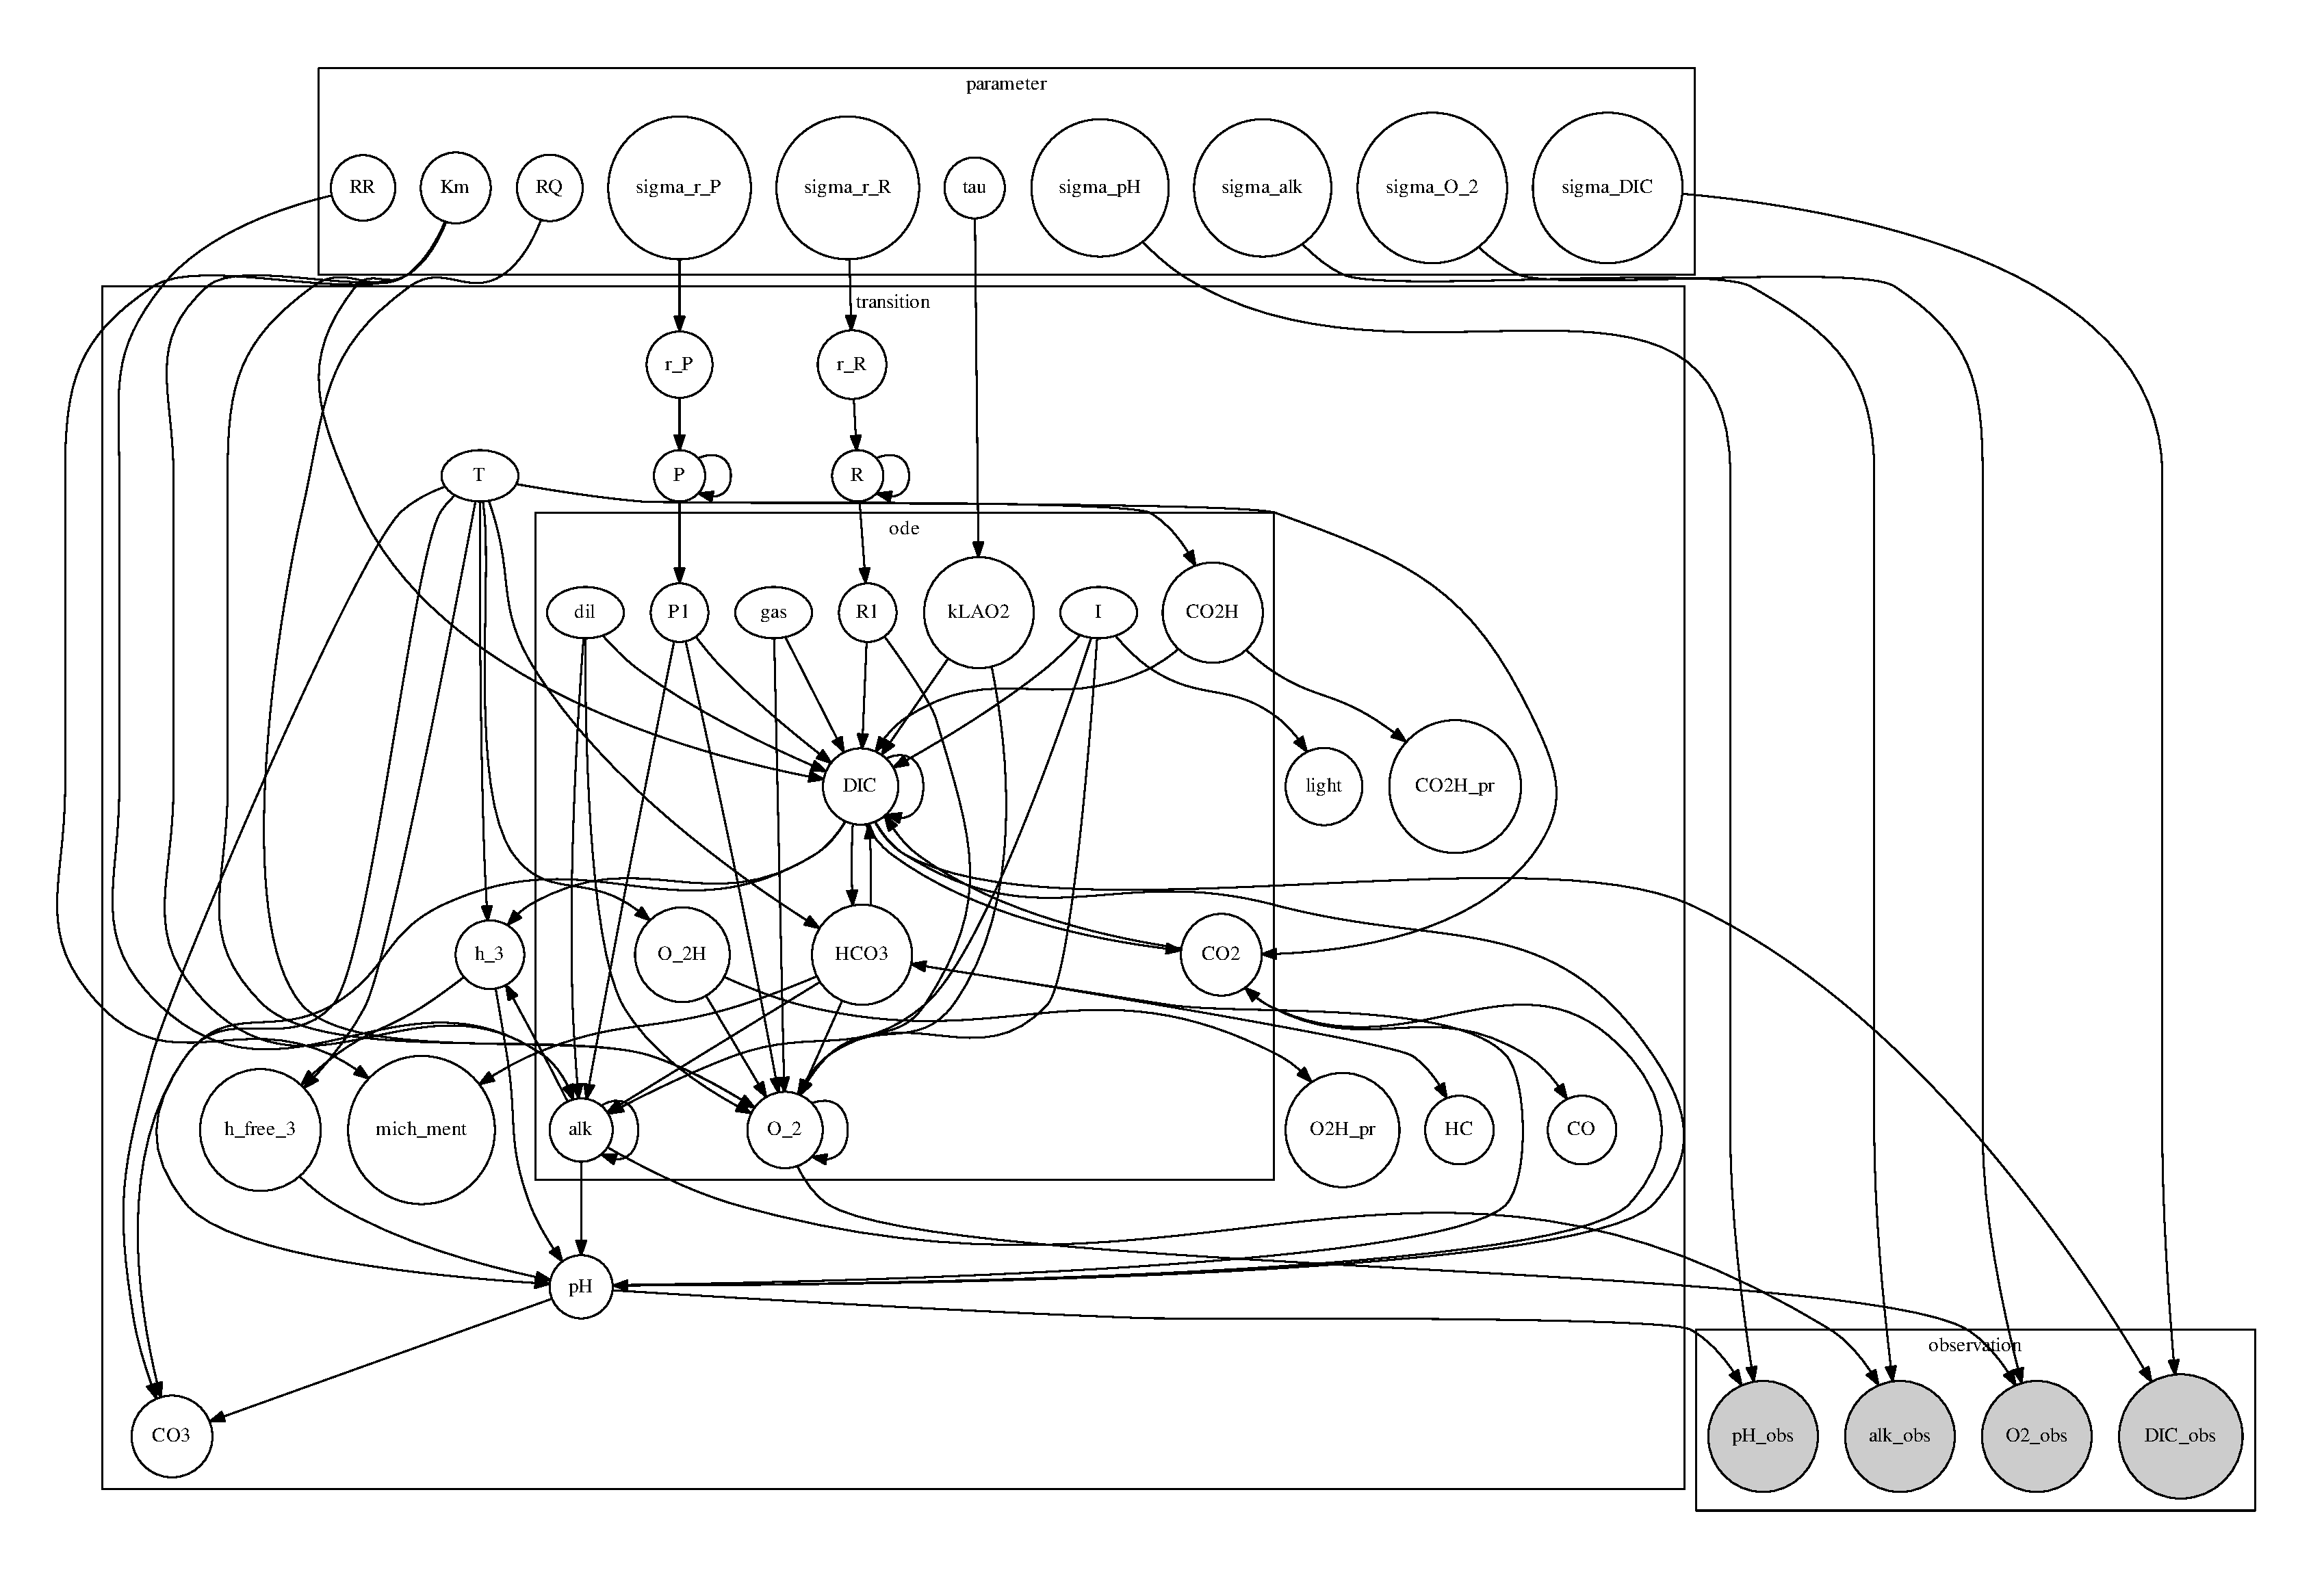
\includegraphics[width=0.9\textwidth]{images_microalgae/micro_template.pdf}}
	\caption[.]{Directed Acyclic Graph of the LiBbi model file micro\_iterative.bi}
	\label{fig:micro_DAG}
\end{sidewaysfigure}


\begin{figure}
	\centerline{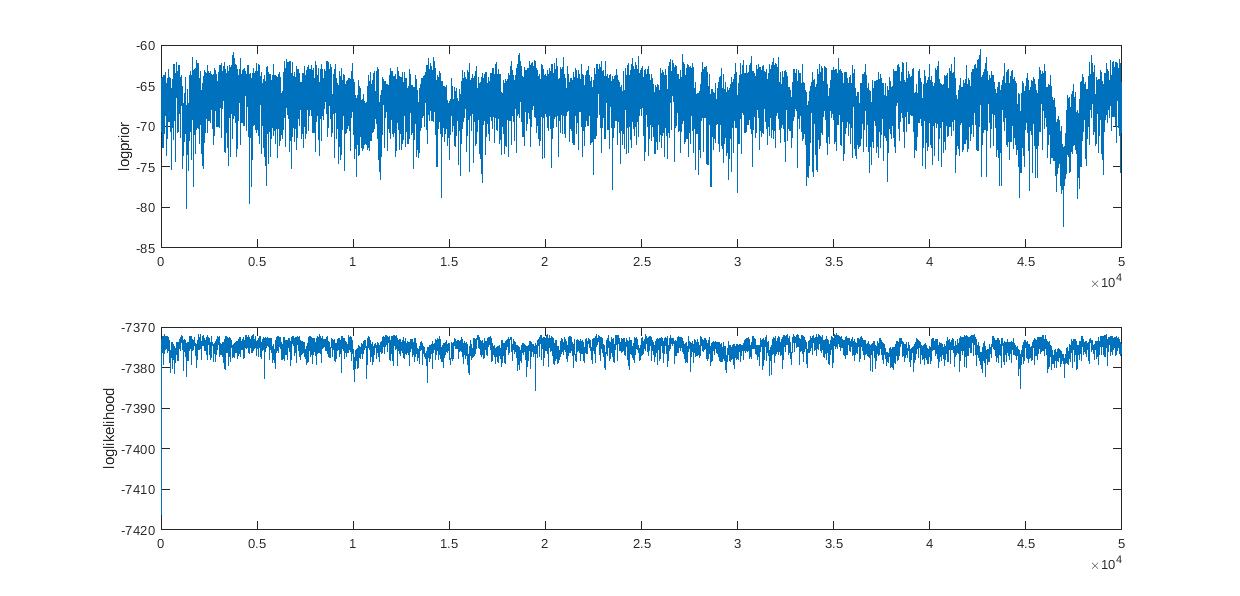
\includegraphics[width=1.3\textwidth]{images_microalgae/posterior_plots_with_fake_data/loglikelihood}}
	\caption[.]{Log-prior and log-likelihood for the simulated data experiment.}
	\label{fig:micro_sim_loglikelihood}
\end{figure}

\begin{figure}
	\centerline{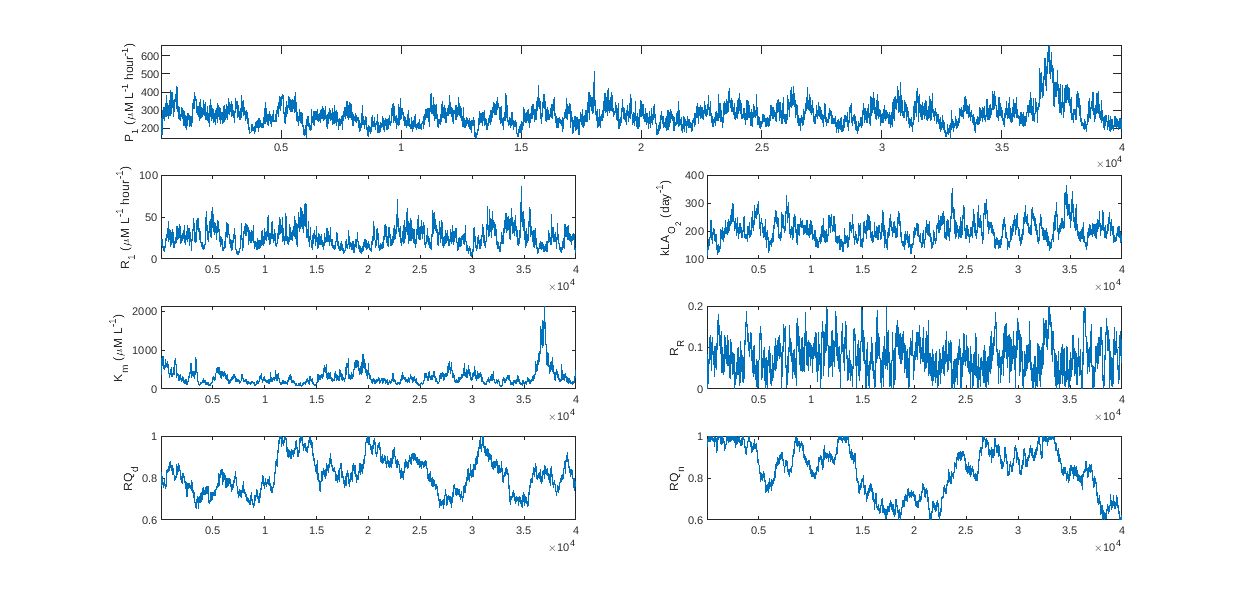
\includegraphics[width=1.3\textwidth]{images_microalgae/posterior_plots_with_fake_data/model_parameters_traces}}
	\caption[.]{Parameter posterior traces for the simulated data experiment.}
	\label{fig:micro_sim_model_parameters_traces}
\end{figure}

\bibliography{seagrassbib}{}
\bibliographystyle{plain}

%\ifx\printbibliography\undefined
%\bibliographystyle{plain}
%\bibliography{bibexport}
%\else\printbibliography\fi



\end{document}

